\chapter{Introduction}
%\section{Cyber physical systems}
Computers have penetrated every aspect of our society. Few things are manufactured today that do not contain a microprocessor or computing device. Many of these digital devices interact with the physical world, making them \emph{cyber-physical systems} (CPS).

One type of cyber-physical system is industrial control systems (ICS). These production systems can be factories or electrical grids, to name a few examples. In the middle of the 20th century, the existing industrial systems started becoming digitalized. First, the programmable logic controllers (PLC) replaced electric switches. Later, the PLCs gained increased sophistication with network capability. 

The first change with the digitalization of industry has been called Industry 3.0. Now, Industry 4.0 is being introduced as the next evolutionary step of the industry. Industry 4.0 is a step towards more automated systems coupled with computing devices. Industry 4.0 will enable optimization of production flows and more efficient production. Much of this is achieved with increased connectivity between parts in the system. The increased connectivity in industrial control systems, together with the proliferation of connected cyber-physical systems, has led to more systems being connected to the internet. While connectivity provides many advantages, it also opens systems to remote attacks. 

The first significant cyberattack against industrial control systems, STUXNET in 2010 \cite{falliere2011w32}, was quickly followed by other attacks \cite{case2016analysis} \cite{giles2019triton}. There can be no doubt that when cyber-physical systems, such as factories, power grids, and water distribution systems, are connected to the internet, they will be subject to attacks.

The industry is well aware that attacks against cyber-physical systems are a real threat; for example, the authors of the Industry 4.0 report \cite{kagermann2013recommendations} lists cybersecurity as one of its key enablers.

In this thesis, we will look at several aspects of security for cyber-physical systems. Our work can be divided into two topics; security lifecycle management for cyber-physical systems and encryption protocols for wireless sensor networks.

On the topic of security management of cyber-physical devices, one work deals with the security management of industrial control systems using Digital Twin. Digital Twin is a concept where a physical device is connected to a Digital Twin. This Digital Twin can be used for a multitude of things; we have focused on how to manage security in complex cyber-physical systems by leveraging a relatively simple State Synchronization protocol.

We also have investigated the topic of Secure ownership transfer for constrained devices. Secure ownership transfer is the process where one entity transfers the ownership of a set of devices to another entity. We have looked at this problem for very constrained devices and designed a solution based on symmetric-key primitives.

Furthermore, in our work on encryption protocols for wireless sensor networks, we have included two publications. In the first publication, we have evaluated the recently standardized protocol OSCORE in terms of efficiency.
In the second paper, we propose an encryption scheme that provides identity privacy for constrained devices in a sensor network when transmitting data to a remote server for analytics.

The nature of cyber-physical devices poses new security challenges. Some are limited in computational power, network capacity, and energy. Other devices such as industrial control systems are not \emph{per se} constrained, but the task of controlling the process with hard real-time deadlines consumes so much of the available resources that any security solution developed for this purpose must be light-weight. The requirement for light-weight solutions is present in all works contained in this thesis.

\section{Dissertation Outline}

 We will discuss the background to industrial control systems in Section \ref{sec:cps}, Constrained devices in Section \ref{sec:constrained_devices}, Object Security \ref{sec:object_security}, Secure Ownership Transfer in Section \ref{sec:ot}, and Digital Twin in Section \ref{sec:digital_twin}. 

The background will then serve as a stepping stone for the papers that we present in Chapter \ref{ch:coc}. The papers themselves follow this introduction.


\chapter{Background}
\label{ch:background}
In this chapter, we will present the background to the research fields treated in the thesis. 
This thesis covers a few different topics, all of them related, although not directly. All publications deal with at least two of these aspects, as presented in the following chapter.

\section{Industrial Control Systems}
\label{sec:cps}
The first automated industrial control system can maybe be said to be the loom developed by Joseph Marie Jacquard in 1804. It can be seen as the first iteration in the evolution of modern systems. It was a primitive computer "programmed" by punch cards to weave patterns in cloth. Since then, automated systems that control physical processes have become increasingly prevalent and increasingly sophisticated. The technological evolution has gone from pneumatic systems through electro-mechanic systems to digital systems.
Virtually everything on a modern factory today is automated. This automation has increased efficiency and the precision of machinery.

But a second technological revolution has happened in parallel to the automation of the industry.
The first device connected to the Internet was a vending machine at Carnegie Mellon University in 1982. Almost 40 years later the number of cyber-physical devices is projected to reach 75 Billion by 2025\footnote{https://www.statista.com/statistics/471264/iot-number-of-connected-
devices-worldwide/}. 

Modern industrial control systems are an amalgamation of information and communications technology and the evolved automation systems used in the industry. 

Sometimes during the 1980s, drawbacks were identified with having isolated industrial control systems (ICS) \cite{wollschlaeger2017future}. Connecting manufacturing systems and distribution systems with the organization's Enterprise Resource Planning systems (ERP) was desired. This integration of ICS systems and traditional IT systems have increased the efficiency and agility of process control. Complex systems have been enabled, such as Supervisory Control And Data Acquisition (SCADA). Another benefit is the ability to configure or control processes and machines remotely.

However, this has opened a new attack surface in the form of remote attacks. We will describe the security aspects of ICS shortly. First, we will give the reader an overview of the differences between IT environments and ICS environments to provide a better understanding of the security implications.


Figure \ref{fig:nist_ics} shows the main parts in an industrial control system, according to NIST \cite{stouffer2011sp}. The most important part of the system is the controlled process; without a process to control, there are little use for a control system and its associated parts. The Controller uses input values from sensors, which can be, for example, temperature sensors or flow-meters. These input values are used by the Controller to calculate commands that the Controller then sends to actuators. Actuators can be valves, pumps, and industrial robots. The actuators, in turn, alter the physical properties of the controlled process to give the desired results. 

The whole controlled process is, although automatic, still supervised by a human operator using a Human-Machine Interface (HMI).
From the HMI, an operator can modify the setpoints and monitor the status of the process. Part of the HMI is also an easily overlooked part but essential for safe operations, the STOP mechanism. The stop buttons are not only found on the screens in the control rooms but also as big red buttons scattered around the premise. 

Lastly, most systems today are connected to remote diagnostics and maintenance systems. These systems can be used to control the process remotely and to collect and process data, not only about the process but also about each part in the system, such as individual robots and machines. 

\begin{figure}[ht]
\centering
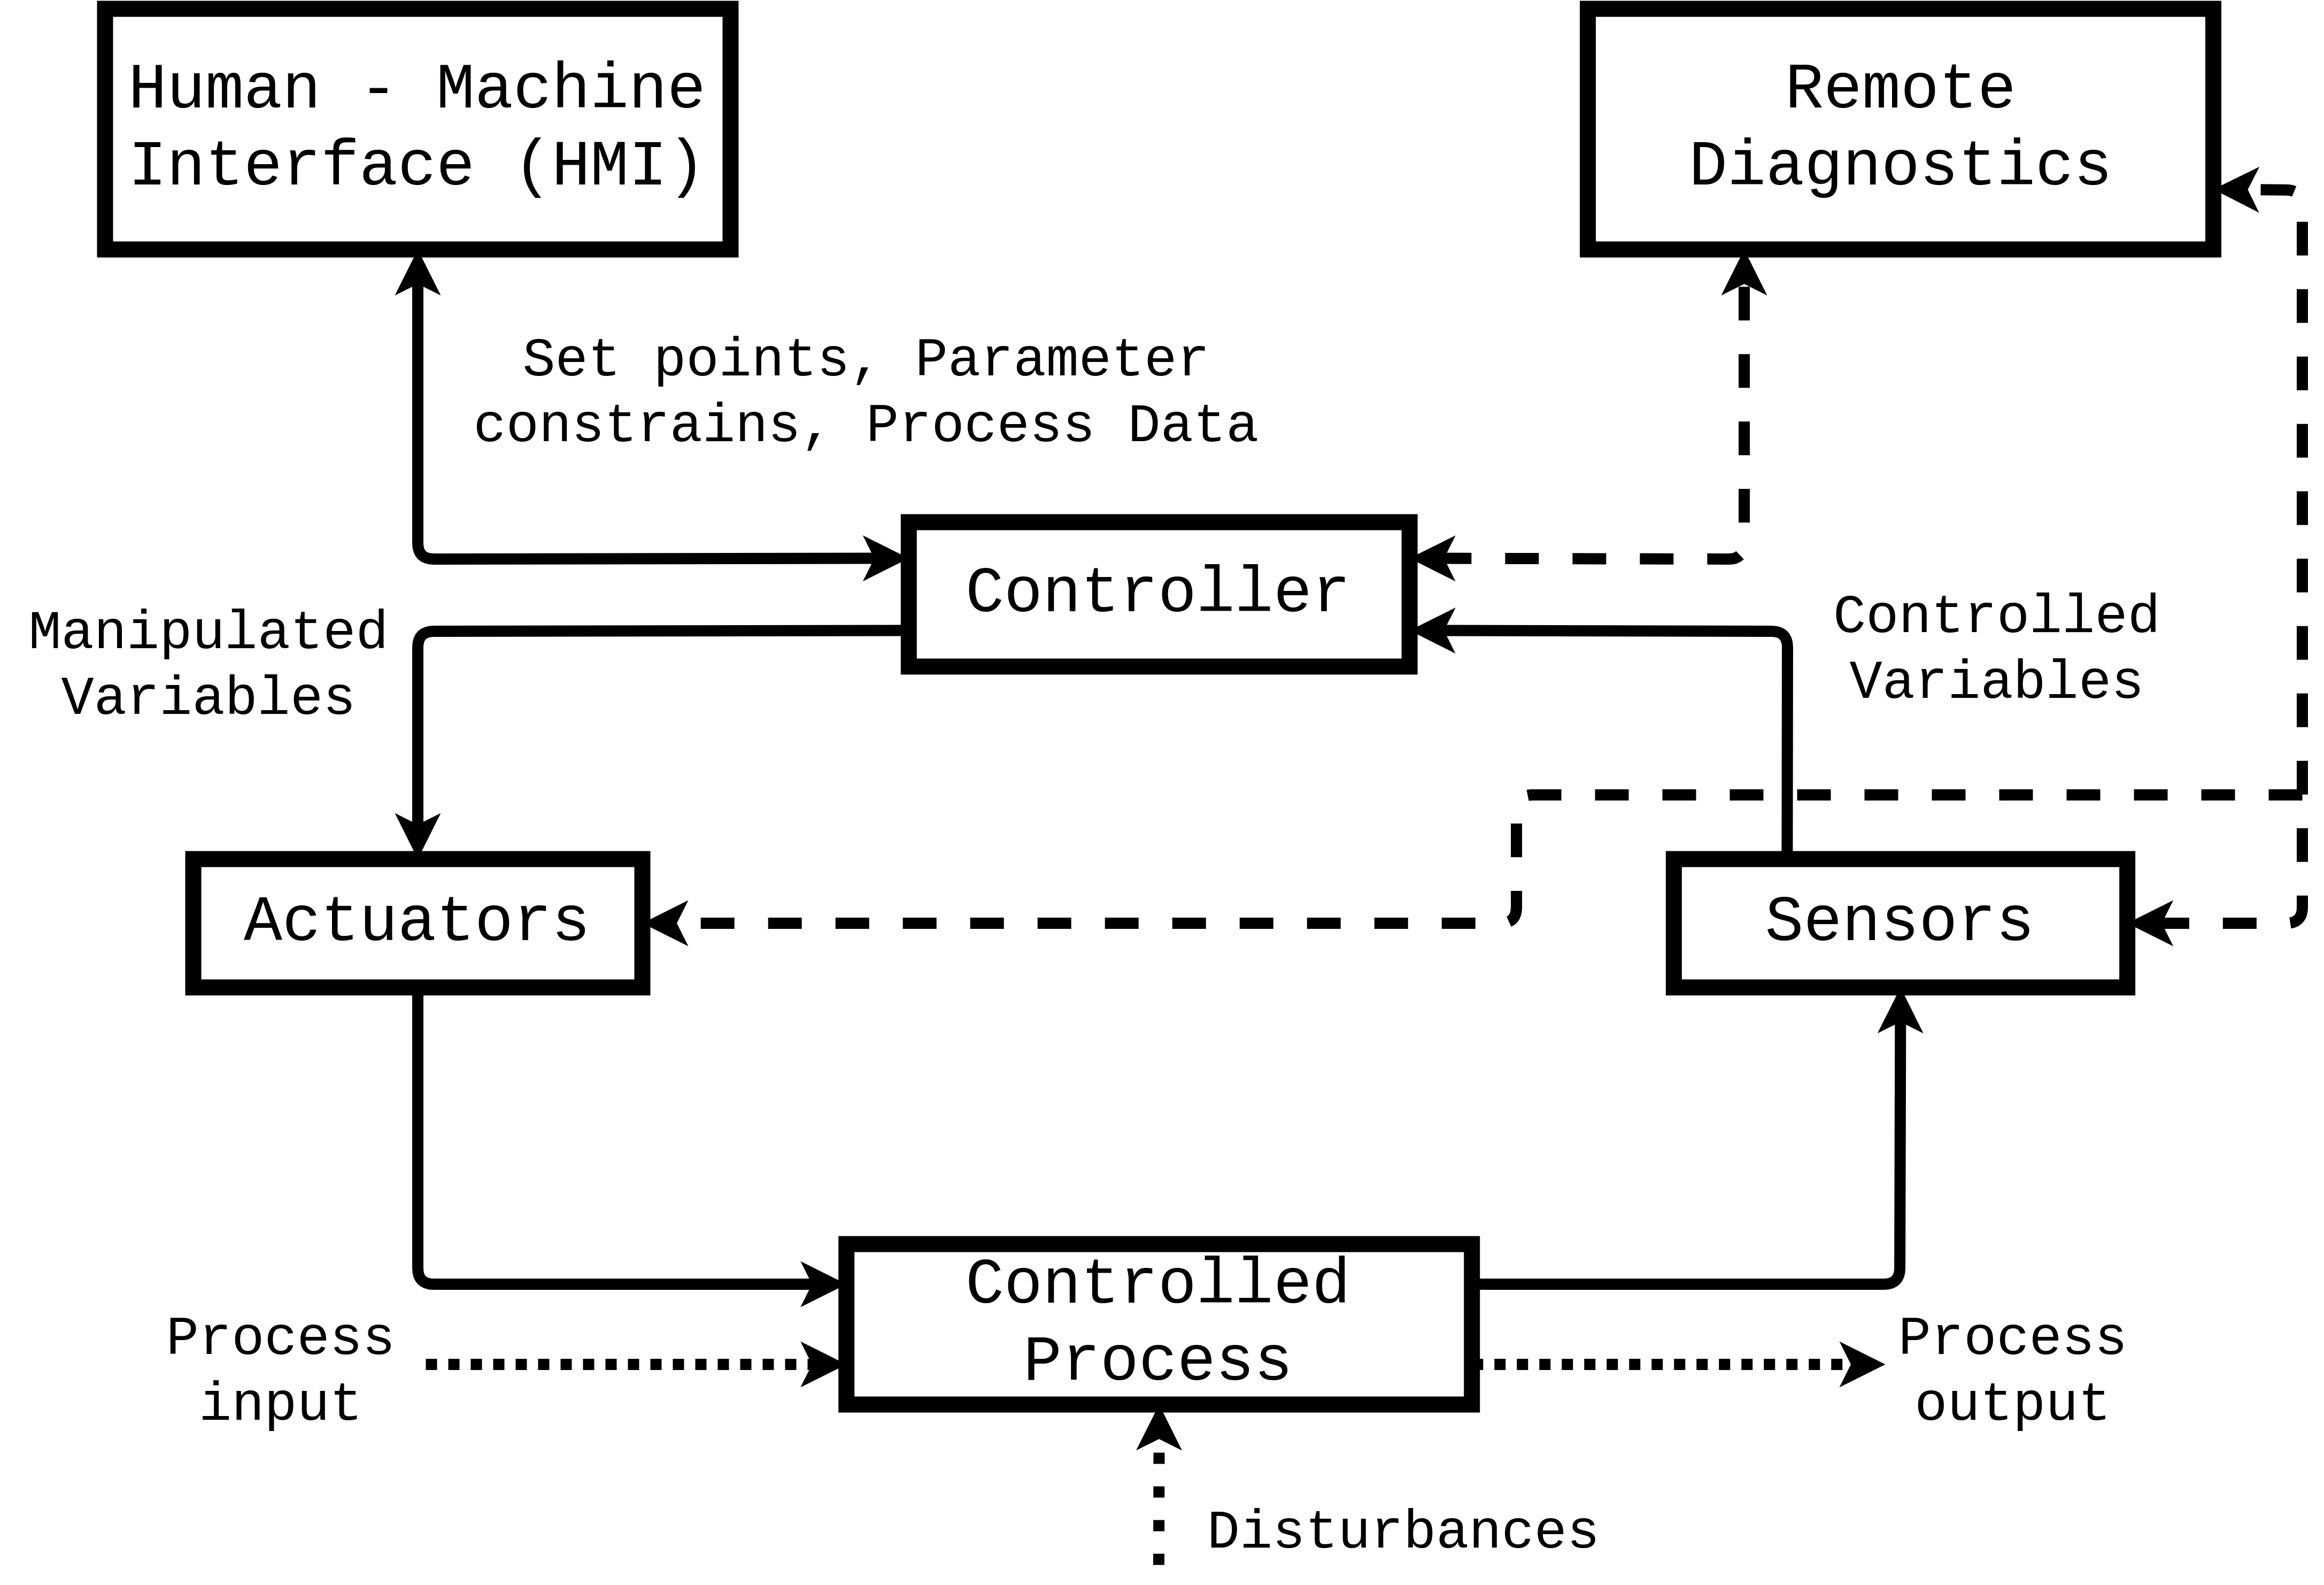
\includegraphics[width=0.8\textwidth]{images/NIST_800.png}
\caption{ICS operation according to NIST, from NIST Special Publication 800-82}
\label{fig:nist_ics}
\end{figure}

Figure \ref{fig:nist_ics} can show an abstract representation of an ICS system. The process in Figure \ref{fig:nist_ics} can be either a small pump process or an entire factory. We can see that the model presented is limited in its applications. 

A more detailed model, made to represent a total view on an ICS deployment, is the Purdue Model \cite{williams1992purdue}. The Purdue Enterprise Reference Architecture, as is its full name, was developed in 1990 by members of the Industry-Purdue University. The model is shown in Figure \ref{fig:perdue}; it gives a hierarchical view of different parts of an ICS system. 

Starting at the bottom with Level 0, we have the devices that form the interface between the physical process and the control system, which are sensors, actuators, and robots, that contain both sensors and actuators. At Level 1, we have different systems of local control, continuous and discrete control of processes and, also the essential safety control. Moving up to Level 2, this is the highest level in what is called a Cell, we have the Human-Machine Interfaces (HMI) and Engineering Workstations. A plant can have more than one Cell. At Level 3, the systems that manage the Cells are located; this is also where the site operations and manufacturing operations systems are. 

Above Level 3 is the Demilitarized Zone (DMZ). This area separates the critical and sensitive parts of process from the rest of the IT environment of the organization. The DMZ is separated from both sides by firewalls that filter the network traffic flowing through DMZ. The idea behind the DMZ is to have no direct connection into or out from the Levels 3 and below. If remote access is used in a system, this is where gateways for a remote access system is situated. Level 4 and 5 are where traditional IT resides, email servers, the Intranet, and business planning are located here.

\begin{figure}[ht]
\centering
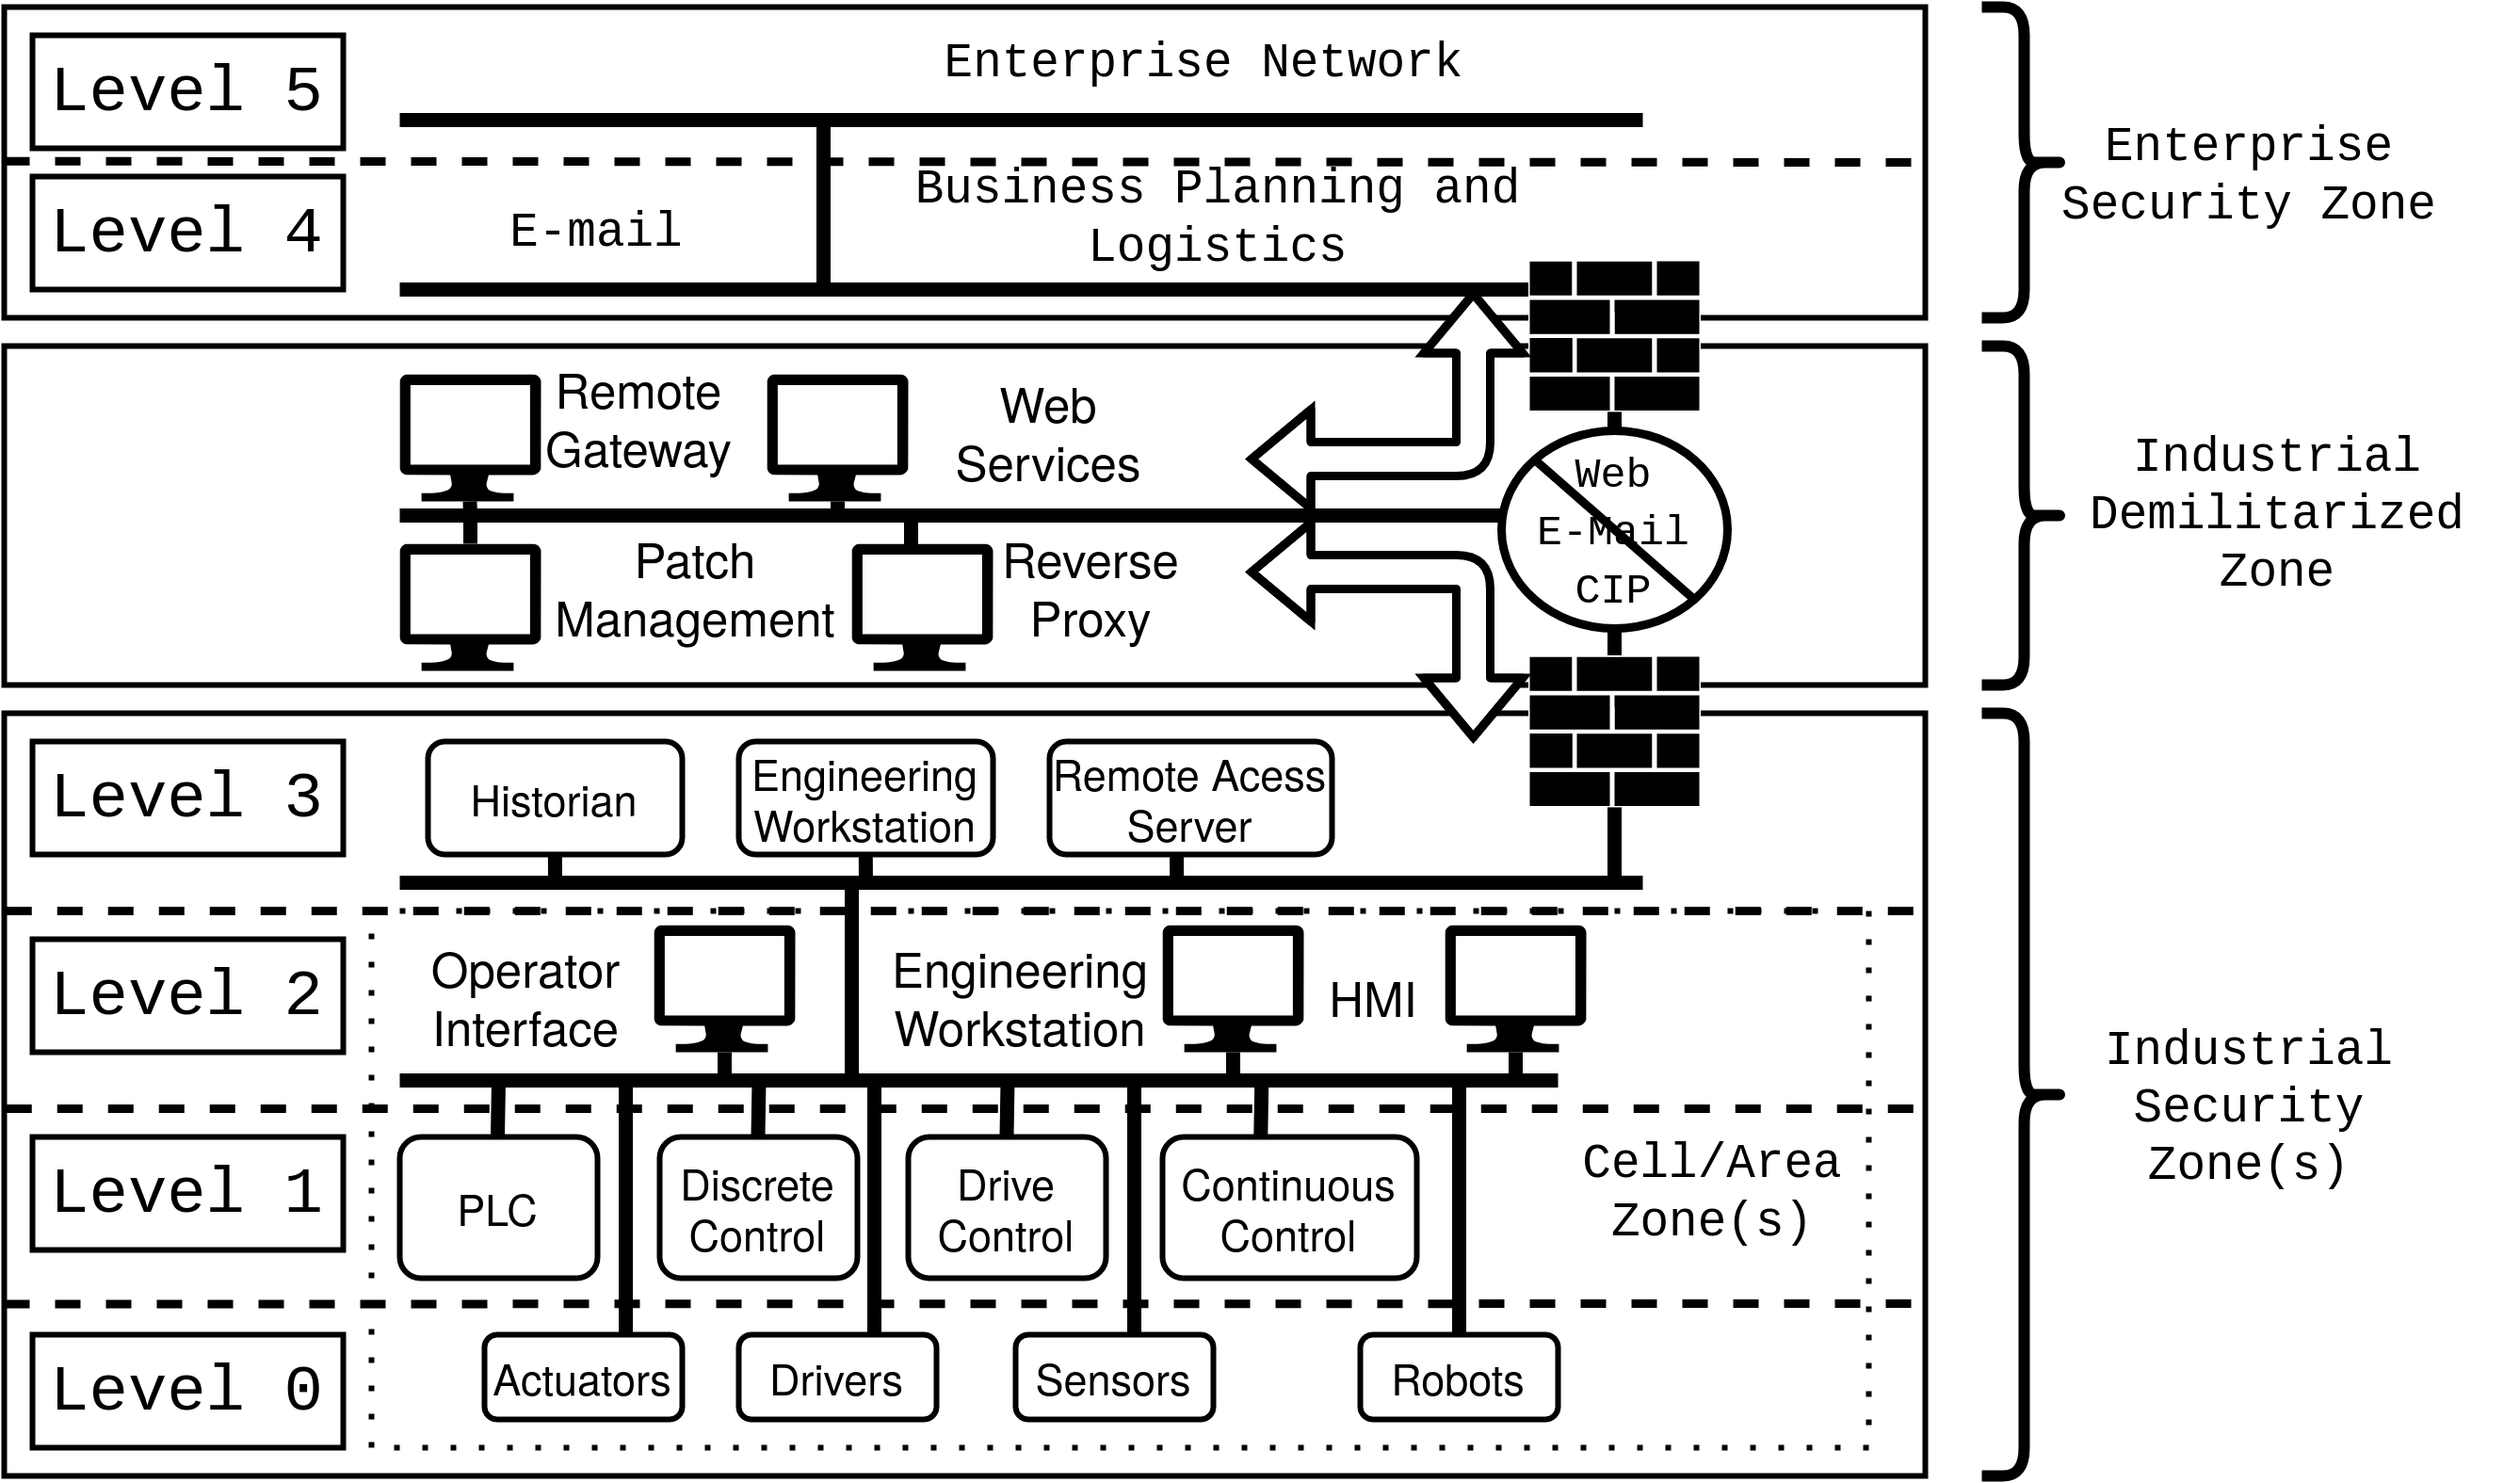
\includegraphics[width=\textwidth]{images/purdue.png}
\caption{The Purdue Enterprise Reference Architecture, a model for ICS.}
\label{fig:perdue}
\end{figure}

Perhaps the most crucial difference between IT and ICS is that in industrial control systems, the \emph{process} is the end goal. The process generates value by producing something; thus, it gets prioritized when resources are limited.

Another key technical difference between familiar IT systems and ICS systems is the aspect of real-time tasks in ICS. A process that controls, for example, a chemical process or an electricity grid, cannot have too high latencies. A correct control signal that arrives too late is of no use. In IT, there is often no need for real-time deadlines. Most IT systems process data at the request of a user; as long as the user perceives the system as responsive, the performance is good enough.

Close to the aspect of real-time deadlines is the property of availability; it is easier to have redundancy in an IT system. Multiple instances of a cloud server with a load-balancer can keep a service available even when parts of the system is undergoing maintenance. But in ICS, an outage can have severe consequences, e.g., an electricity grid or drinking water supply can impact thousands of people. To guarantee the availability of critical processes, the process control system must be available. The control system is often redundant to prevent outages caused by a faulty control system.


It might, therefore, not come as a surprise that the systems used to control different processes are highly specialized systems. Not only as ICS devices but also within the field of ICS control systems for different types of processes have significant differences. There is very little commonality between, for example, a welder robot from a car building assembly line and a phase-controller from an electricity grid. The complexity of the process by itself, together with the specialized systems, makes almost all ICS deployments unique.

Because of the specialization of systems, component lifetimes are long. Systems and parts are expensive, a stop in production to install and deploy a system might be too expensive for an organization. Patches are also slowly applied to systems, not only because of the risk of breaking some functionality but also because a certified system might lose the certification when a patch is applied.

Because ICS devices have been developed in silos separated from ordinary IT devices, the protocols, standards, and technologies used in ICS is different compared to a traditional IT environment. This not only affects the interoperability of ICS and IT systems but also does not let ICS systems take advantage of the development of better IT security protocols and mechanisms.

As we have shown here, many aspects differentiate ICS from IT. Of course, these differences impact security, and we will discuss that in Section \ref{subsec:ics_security}.

\subsection{Industry 4.0 and Next-Generation Manufacturing}
\label{subsec:i4}
Sometimes called the fourth industrial revolution, following the third Industrial Revolution, the digitalization of manufacturing from the mid of the 1900s. Industry 4.0 has become the accepted term in Europe on the next generation of the industry.

In 2012 a German research project presented a set of recommendations to the German government about the future of the industry \cite{kagermann2013recommendations}. The goal of \emph{Industrie 4.0} or Industry 4.0 is to improve productivity. The productivity improvements will be gained from an increase in flexibility, where factories build to demand instead of producing to inventory. A critical factor in achieving this will be collecting, sharing, and spreading information through the factory, together with decentralized decision making.

The list of technologies and concepts that will realize Industry 4.0 is long; among them are IoT, Cybersecurity, Cloud computing, Big Data, and Simulation. Other technologies are listed, such as Augmented reality and Additive manufacturing, but we will focus on the technologies relevant to this thesis.

IoT is a key component of Industry 4.0, used in this industrial setting. Industrial IoT (IIoT) is often used to describe the connected devices in manufacturing systems. In Section \ref{subsec:wsn_iot} we discuss IoT and IIoT. IoT is also key in Paper I, II, and III. 

ICS data collection is needed for advanced analytics and improved production performance, to give two examples. Collecting data from a production environment will often result in large data sets; doing analytics on these big data sets is a whole discipline called Big Data analytics. In Paper II, we look at this collecting of data from a privacy perspective. We have identified the need for Identity Privacy of data items that are transmitted to a server for analytics.  

 
\subsection{Security Aspects of Industrial Control Systems}
\label{subsec:ics_security}
The properties we have described above make it clear that security for ICS faces different challenges compared to IT security. In IT security, the Confidentiality, Integrity, and Availability (CIA) triad is often used \cite{perrin2008cia} to describe the goals in IT security activities. Note that the CIA refers to the \emph{data} used \emph{in} the system and not the system itself.
The data shall be confidential; that is, it shall not be readable by any unauthorized entity. The data shall be integrity protected, which means that an unauthorized entity shall not be able to manipulate the data. Lastly, the data shall be available since data is of no use if it not readily accessible. 

According to several researchers, for example, \cite{Gollmann2016} and \cite{stouffer2011sp}, the CIA security model does not map well to ICS. For instance, while the CIA model considers theft or manipulation of data, in an ICS setting, risk of personal injuries or equipment damage must also be taken into account. See \cite{stouffer2011sp} for a more detailed analysis of this issue.

The availability of systems is more critical in ICS. A production plant can take days to come back online after a stop. The resulting downtime could cause high costs for the owner and operator. 

In this thesis, we have included papers that deal both with traditional security properties, like the above mentioned CIA triad, and security life cycle management. Since outages due to maintenance and cyber-attacks should be avoided, methods for doing security life cycle management in ICS are needed. This security life cycle management must not waste the limited resources in ICS. In Paper IV, we have developed a security architecture using the concept of Digital Twin. Digital Twin are further discussed in Section \ref{sec:digital_twin}, and as shown in the included paper, it is a powerful tool for security monitoring with a low impact on legacy systems and real-time critical systems.

\section{Constrained Devices}
\label{sec:constrained_devices}
The term \emph{constrained devices} or \emph{constrained nodes} can be used to describe computing devices with limited capability, i.e., they are limited in some way. These limitations can be CPU-Power, RAM and ROM memory, network capabilities such as latency and bandwidth, and energy. Energy can be limited because the device is powered by an energy harvesting device such as a solar panel or from a battery. Devices may sleep for periods to save energy and not being able to respond to communication and perform any computation during those intervals.

The Internet Engineering Task Force (IETF) has standardized terminology for these devices \cite{rfc7228}. Because not all constrained devices are the same, IETF has defined several categories that determine \emph{how} limited a device might be. One limiting factor when it comes to performing complex computations; is the size of the available memory. In Table \ref{tab:constrained-classes}, we show the categories of constrained nodes as defined by IETF. Why they use memory instead of a metric such as CPU-speed, is because memory size results in a more substantial factor of the final cost of a device. Memory takes up a lot of space on the semiconductor die, and the size of the die directly influences the price \cite{koopman2015}.


The effect of these memory limitations is that a memory-constrained device is only capable of doing a small set of computations. A small amount of ROM limits the amount of code that can be present in the system, thus only a select few tasks can be done. A small amount of RAM limits the number of intermediary states and the size of the data that can be handled. For example, in a protocol such as Datagram Transport Layer Security (DTLS), RAM limitations directly limit the number of security contexts, which in turn limits the number of simultaneous connections the device can handle.

\begin{table}[ht]
\centering
\caption{Classes of constrained devices according to RFC7228.}
\label{tab:constrained-classes}
\begin{tabular}{lll}
\hline\hline
\textbf{Class}  & \textbf{Data Size (RAM)}  & \textbf{Code Size (ROM)}    \\ \hline
Class 0, C0 & \textless{}\textless 10 KiB & \textless{}\textless  100 KiB \\ 
Class 1, C1 & $\sim$10 KiB                & $\sim$100 KiB                 \\ 
Class 2, C2 & $\sim$50 KiB                & $\sim$250 KiB                 \\ \hline\hline
\end{tabular}
\end{table}


Apart from memory constraints, energy is one important aspect to consider when evaluating the capabilities of a system. It is no surprise that running a CPU, peripheral, and a radio-modem consumes energy. Constraints of energy have significant ramifications when a system is designed, energy-efficient CPUs are generally less powerful, and the same goes for peripherals and radio-modems. IETF has put the energy constraints on a scale from 0 to 9, where 9 is no limitation, and 0 is energy harvesting. 

The different categories can be seen in Table \ref{tab:energy-constraints}. For example, an E9 device can be an Ethernet-enabled surveillance camera that is powered by Power over Ethernet. A class E0 device is, for example, an RFID-tag that harvests energy when a reader interrogates it, this small amount of energy harvested is then used to send a reply. 

Since constrained nodes might be sleeping periodically, communication is often asynchronous. The lower layer MAC protocols handle radio duty-cycling and make sure that the receiving node is powered on when it is going to receive messages.


\begin{table}[ht]
\centering
\caption{Classes of energy constraints according to RFC7228.}
\label{tab:energy-constraints}
\begin{tabular}{lll}
\hline\hline
\textbf{Class} & \textbf{Type of energy limitation}  & \textbf{Example Power Source}                               \\ \hline
E0    & Event energy-limited                      & Event-based harvesting                             \\ 
E1    & Period energy-limited                     & Periodically recharged battery                   \\ 
E2    & Lifetime energy-limited                   & Non-replaceable primary battery                    \\ 
E9    & No limitations to available energy           & Mains-powered                                      \\ \hline\hline
\end{tabular}
\end{table}

\subsection{Security Aspects for Constrained Devices}
After describing the capabilities and limitations of Constrained devices in the previous section, we will now discuss the implications for security.
Because of the limitation in CPU-power, memory, energy, and network capabilities, traditional security solutions developed for desktop and server computing environments can prove unsuitable. The limited performance of constrained CPUs make public-key encryption time and energy-consuming, hardware-acceleration can be utilized to make it more feasible.

Traditional x509 certificates might require too much bandwidth and memory to be stored in RAM in a device. Research has been done to reduce these numbers \cite{forsby2017lightweight}, but also with limited network capability; it might be difficult to validate an entire certificate chain, thus severely limiting the usefulness of certificates.

The ubiquitous protocol for secure communication in traditional IT Transport Layer Security (TLS) \cite{RFC8446} uses TCP as the underlying transport mechanism. Sessions are not desirable when constrained devices communicate asynchronously. Instead, DTLS is standardized as an alternative to TLS. DTLS uses UDP as the underlying transport; this removes the need for TCP sessions. Using UDP also reduces the overhead of each transmitted packet.

The security protocols and solutions developed for constrained devices must consider these limitations \cite{I-D.irtf-t2trg-iot-seccons}. Security solutions must be resource-efficient. Limiting message overhead to save bandwidth and energy is a requirement. When selecting cryptographic primitives, efficient algorithms must be prioritized. This means using symmetric-key encryption where it is possible and limiting the use of public-key cryptography. Reducing the transmitted message size is also an essential goal since sending and receiving data consume energy. The protocol OSCORE, recently standardized by IETF, was designed with low message overhead as one of the design goals \cite{RFC8613}. We have evaluated the efficiency of the OSCORE protocol in Paper III; we investigate message overhead and energy consumption to examine the efficiency of the protocol. 

In Paper I, we have developed a Secure ownership transfer protocol for very constrained devices. The protocol we have designed uses symmetric cryptography and results in an efficient protocol. The topic of Secure ownership transfer will be described in detail in Section \ref{sec:ot}. In Paper II, we have designed a protocol that gives Identity privacy for sensor data; the protocol is designed using Object security principles. Object security and identity privacy is described in Section \ref{sec:object_security}. This protocol is also using symmetric cryptography to achieve the stated efficiency requirements. 

\subsection{Wireless Sensor Networks and Internet of Things}
\label{subsec:wsn_iot}
Wireless sensor networks are a designation for a network of, often constrained, devices that communicates with wireless technology. The purpose of the network is often to collect sensor readings from several different places and collect the data for further processing in a central server. 
The shrinking of processors and the decrease in the price of micro-controllers and associated devices have made it possible to deploy sensors with a microcontroller and some kind of networking capability very cheaply. Often these systems are powered by a battery, combined with the need to keep costs down the resulting systems can usually be classified as Constrained devices, as described in Section \ref{sec:constrained_devices}. 

Internet of Things has become the catch-all term for all kinds of connected devices. Everything from a factory connected to a SCADA network to a refrigerator with WiFi can be called an IoT device. Sometimes distinctions are made such as Industrial IoT (IIoT) for connected devices used in an industrial setting. The difference between IIoT and connected control systems described in Section \ref{sec:cps} is that IIoT has a more direct connection to computing resources such as a cloud environment \cite{mclaughlin2016undiscovered}. An IIoT deployment will differentiate from the Purdue reference model we showed in Figure \ref{fig:perdue} in that an IIoT deployment will have a direct connection between the edge devices and the cloud. There is no DMZ in IIoT, like the one that can be found in the Purdue model.


\begin{figure}[ht]
\centering
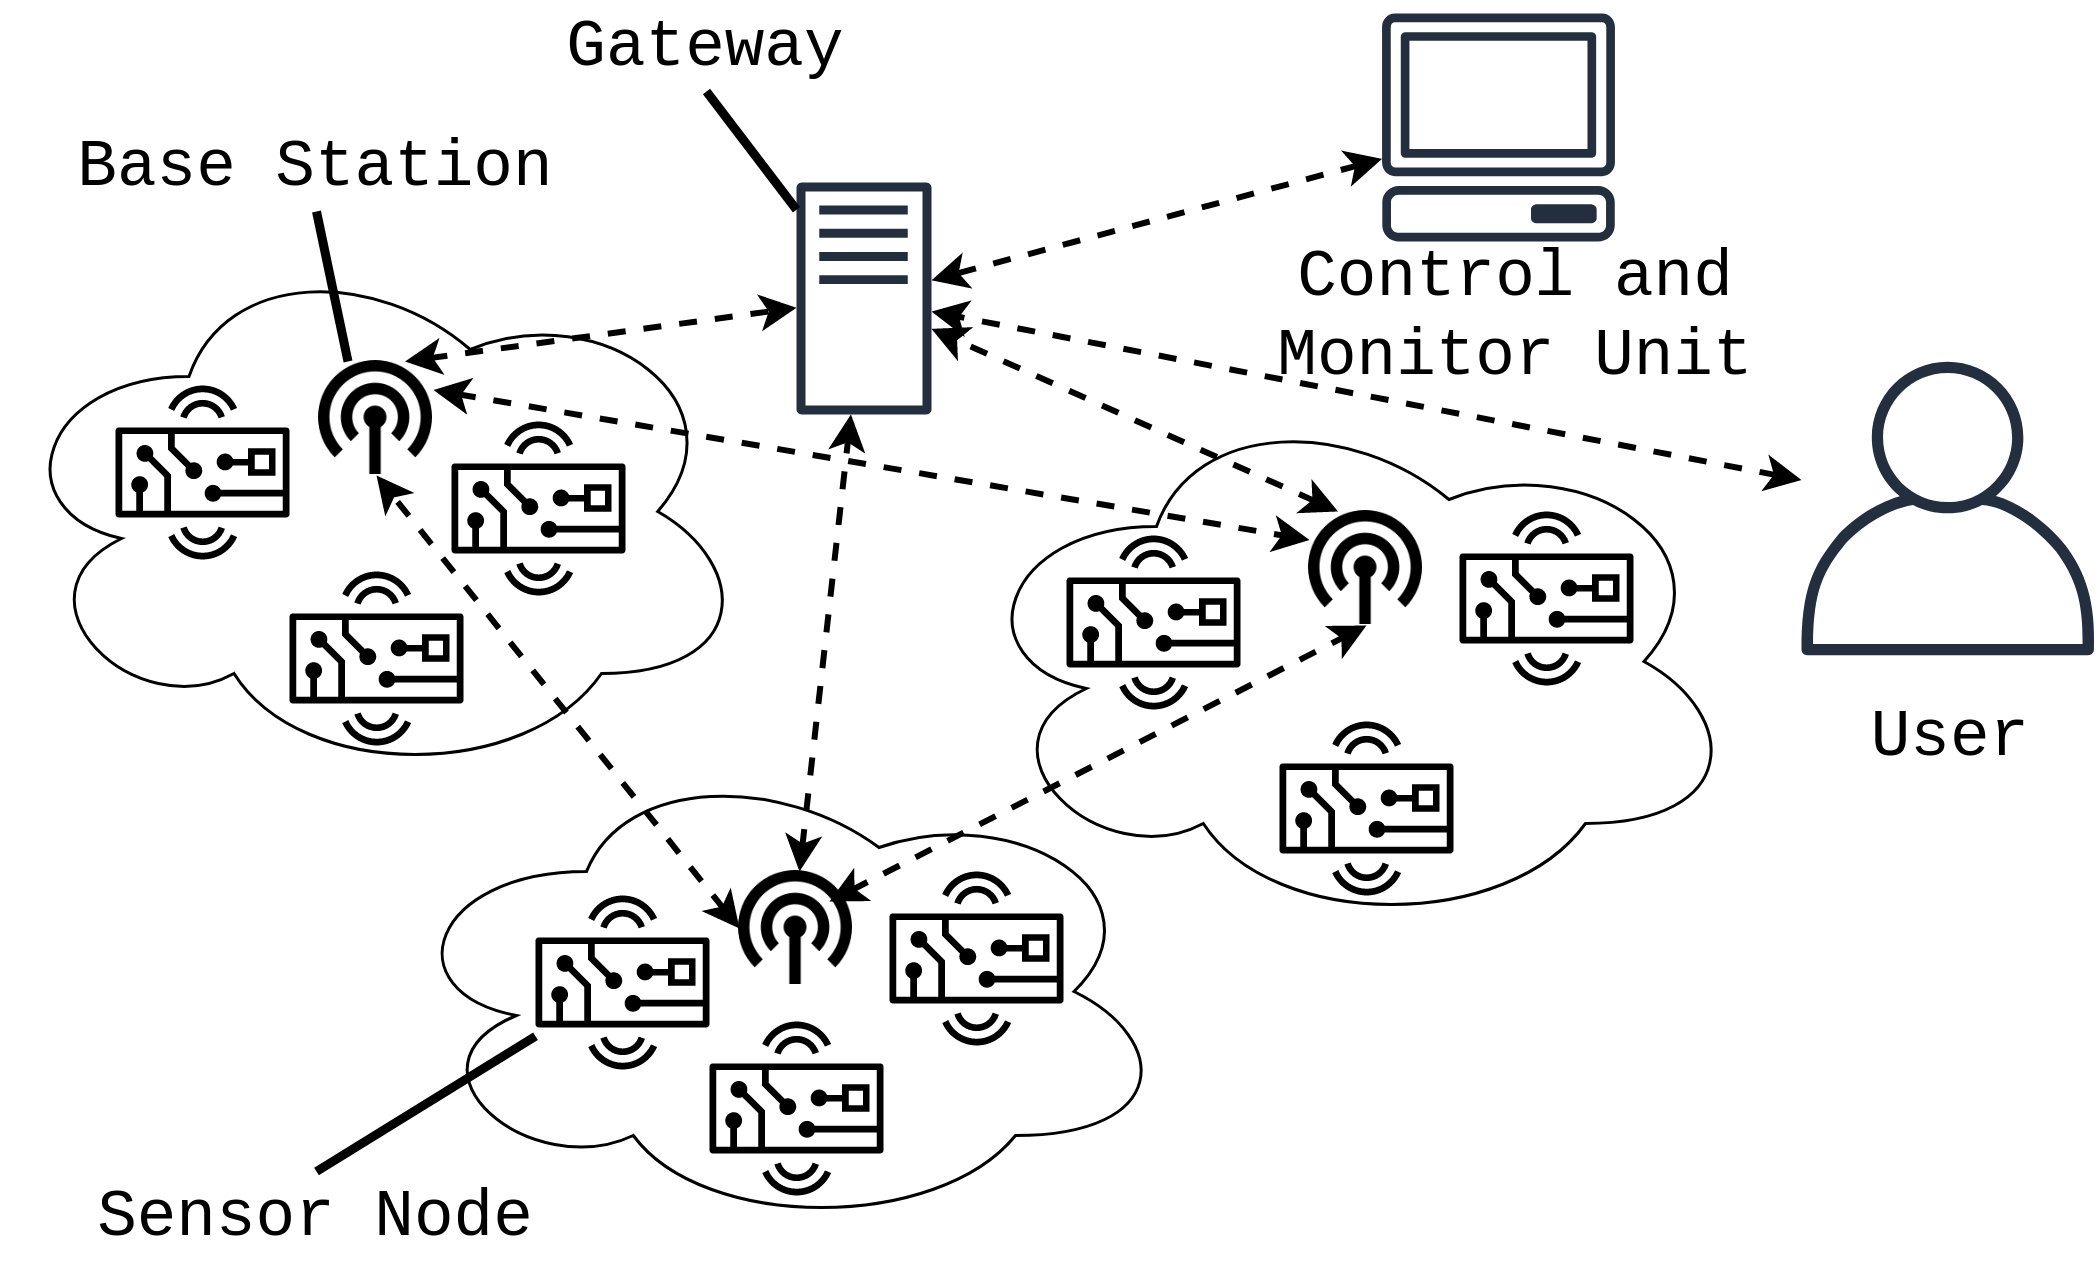
\includegraphics[width=0.9\textwidth]{images/WSN.png}
\caption{A schematic of a Wireless Sensor Network in an industrial setting.}
\label{fig:wsn}
\end{figure}

\subsubsection{Communications Standard for Wireless Sensor Networks}
Many actors have developed Wireless Sensor Networks; as a result of this, there exists a large number of communication protocols and network stacks. WiFi, Bluetooth \cite{haartsen2000bluetooth}, Bluetooth Low Energy (BTLE) \cite{heydon2012bluetooth} and Zigbee \cite{alliance2010zigbee} all use the unlicensed 2.4 GHz frequency band. LoRa \cite{sornin2015lora} uses unlicensed frequencies in the sub-gigahertz range to increase the range compared to the protocols in the 2.4 GHz band. NB-IoT\cite{ratasuk2016nb} uses optimized cellular technology and base stations to achieve wide coverage.


Several application layer protocols exist, the two most common is MQ Telemetry Transport (MQTT) \cite{hunkeler2008mqtt} and Constrained Application Protocol (CoAP) \cite{rfc7252}. MQTT is of type publish-subscribe; clients subscribe to topics, and publishers publish data to these topics. Message brokers then act as intermediaries to forward the data from the publishers to the relevant subscribers.
MQTT is usually transmitted over Transmission Control Protocol (TCP), and TLS is used to secure TLS connections and, in extension, MQTT.
CoAP is a RESTful protocol like Hypertext Transfer Protocol (HTTP). It is transmitted over User Datagram Protocol (UDP), and the most common way of securing it is with DTLS. In this thesis, we have evaluated OSCORE, an alternative approach to securing CoAP. OSCORE uses a security concept called object security that we introduce in Section \ref{sec:object_security}.

\section{Object Security}
\label{sec:object_security}
The earliest reference to Object Security was made in 1995 in RFC1848 \cite{RFC1848} titled \textit{MIME Object Security Services}. The document details how Multipurpose Internet Mail Extensions (MIME) objects shall be encrypted and processed. MIME is a standard that relates to email. Encrypting each mail in a self-contained object is a good solution. The sender can not know if the recipient can receive the email at the time of sending, this means that setting up a secure session to the recipient does not work. The problem with the recipient not being available at the time of sending is solved by using intermediate servers that store and forward the emails. Protecting each mail in a self-contained object eliminates the need for secure sessions between the intermediate servers.

One schematic diagram of an object security message can be seen in Figure \ref{fig:object-security}. It does not show any actual message format, but rather a sample of some fields that might be present in such a structure. What differs between formats and standards, not shown in the figure, is encoding. 

\begin{figure}[ht]
\centering
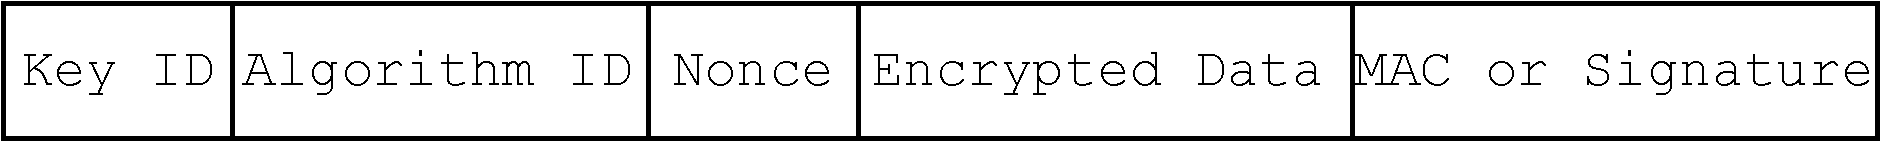
\includegraphics[width=0.9\textwidth]{images/object_security.pdf}
\caption{A schematic of a message or data item protected with object security.}
\label{fig:object-security}
\end{figure}


Object security is a good fit for when a device sends messages to several receivers. Transmitting is only done at intervals, thus object security eliminates the need for keeping a session alive. 
Apart from email, wireless senor networks and constrained networked devices have proved a good fit for object security. Because of the energy limitations and constrained nature of devices, messages are only sent sporadically.

Object security has also been used in web contexts, such as JavaScript Object Notation (JSON) Web Signatures (JWS)\cite{jones2015json}, JavaScript Object Signing and Encryption (JOSE)\cite{barnes2014use} also XML encryption\cite{imamura2013xml}. A similar standard to JOSE is CBOR Object Signing and Encryption (COSE)\cite{schaad2017cbor}.  CBOR stands for Concise Binary Object Representation and has been standardized by IETF as a more compact alternative to JSON\cite{rfc7049}. The difference between JOSE and COSE is the encoding, JOSE uses JSON while COSE uses CBOR. Due to the compact serialized format of CBOR, COSE is more compact than JSON \cite{kalvoda2015implementace}.

One benefit of the object security concept is that it can be used to provide end-to-end encryption. If a message takes a winding route to its destination, encrypting the message in a self-contained way is a practical solution to protect the contents until it arrives at the destination. This is why PGP and all other email encryption schemes work so well; encrypted email can travel between many email-servers until they arrive at the receiver. The receiver, provided they possess the correct keys, can then decrypt the message. These schemes and protocols are quite old now, but they are still used in email applications today. 

Perhaps the first implementation of object security for a constrained wireless device can be found in \cite{brown2000pgp} were the authors port Pretty Good Privacy (PGP) to a Research In Motion (RIM) pager. The RIM pager has more memory than a Class 2 constrained device, but it is still a relatively limited device, considering it uses a 10 MHz Intel 386 CPU from the 1990s. In the paper, they find that Elliptic curve cryptography (ECC) can be done in a couple of seconds. Elliptic curve cryptography is a type of public-key algorithms that require smaller keys and less computation than alternative algorithms for a given level of security. These qualities make ECC suitable for use in constrained devices. The authors argue that the performance of ECC can be acceptable for an email solution.

One more recent application for object security is end-to-end security for instant messaging apps. Asynchronous communication makes this method of encrypting messages a suitable solution. The person you send a message to might not have a direct connection to you. Instead of setting up a secure channel, encrypting the message in a self-contained way, and sending it through intermediaries that do not possess the key, give end-to-end security for the message. 

This use-case is very similar to the problem statement behind OSCORE. Messages pass through intermediate proxies and middle-boxes, the receiving server might be sleeping to preserve energy. Because of this, setting up a secure session is not desirable since a client would have to wait until the sever wakes up.  

Even if object security can solve some security issues, one issue that remains is identity privacy. A message to a receiver like a message shown in Figure \ref{fig:object-security} can have the origin revealed by the Key ID. A server that receives messages from many sources must be able to choose the correct key to decrypt messages. To enable the server to select the right key for decryption, a readable Key Identifier must be present. However, a malicious entity can also read this Key Identifier. Since symmetric keys are shared between only a single pair of communicating entities, knowing the Key ID and the receiver, knowing the sender is trivial. 

Having readable key identifiers is a privacy problem, if a malicious adversary can learn what messages originate at a particular device or person, learning that specific entity's patterns become likely, for some application, this might not be a problem. In others, however, it might reveal patterns about the originating device. Information might be deduced from encrypted messages, even if the contents of which are not known, by analyzing when messages are sent and where they originate. One possible solution to this would be to encrypt either the entire message or just the Key ID with the recipient's public key. Doing that, only the intended recipient can decrypt the message. Using public-key cryptography might, however, be too resource-intensive for some devices.

\section{Secure Ownership Transfer}
\label{sec:ot}
Secure ownership transfer is the process of transferring the control of a secure system from one entity to another. The general premise is that each device has some kind of key or credentials; these keys and credentials are shared with the owner. Some kind of server usually represents the owner. Here we will stick to using \emph{key} for any such credential.

The process of transferring the keys from the old owner to the new is not a suitable solution. The terms \emph{New owner privacy} and \emph{Old owner privacy} have been used to describe desirable features \cite{taqieddin2018tag}. Old owner privacy is that the new owner shall not be able to decrypt recorded traffic and access data from the old owner. New owner privacy is that the old owner shall not be able to learn secrets from the new owner after the transfer is complete.

The topic of ownership transfer has been studied both for IoT and networked devices but more intensively for RFID-tags. RFID-tags are a relevant problem because RFID-tags attached to things, such as parcels, change hands, and move around. RFID-tags can be read remotely close by the tag; this has raised privacy issues. In \cite{juels2006rfid}, the author describes a scenario were RFID-tags carried on a person can be read to reveal sensitive information about their owner. Using keys to enable authorization of RFID-tag access and encryption of the data in transmission has been proposed as a solution to this privacy issue. 

When items with RFID-tags that use keys to authorize reading and provide encryption of the transmitted data change hands, the new owner must be able to access the RFID-tag after the transfer. Ownership transfer is the name given to this problem. The first publication that tries to solve this problem was \cite{saito2005reassignment}. 
Several approaches for ownership transfer exists, protocols have been proposed for single tag transfer or multiple tag transfer. There is also another aspect of proposed solutions, with protocols featuring a trusted third-party and protocols only involving the old and new owner. 

A schematic view of RFID deployment and ownership transfer can be seen in Figure \ref{fig:rfid-ot}. One crucial property for RFID-tags is that they are only powered on when they are read, i.e., interrogated. The RFID-tag reader is an essential part of the system since that is the only device that can directly read the RFID-tags. The RFID-tag reader is usually able to do more advanced computation and is not usually limited in energy. Thus it can be used in the system to perform more complicated calculations.

\begin{figure}[ht]
\centering
%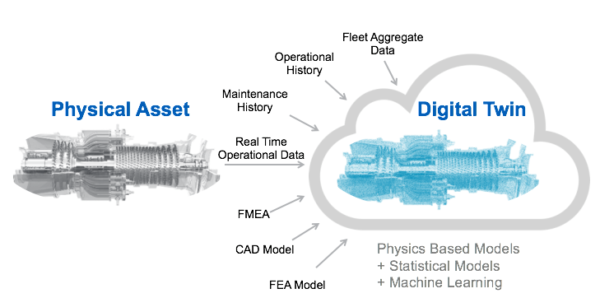
\includegraphics[width=0.9\textwidth]{images/digitial-twin.png}
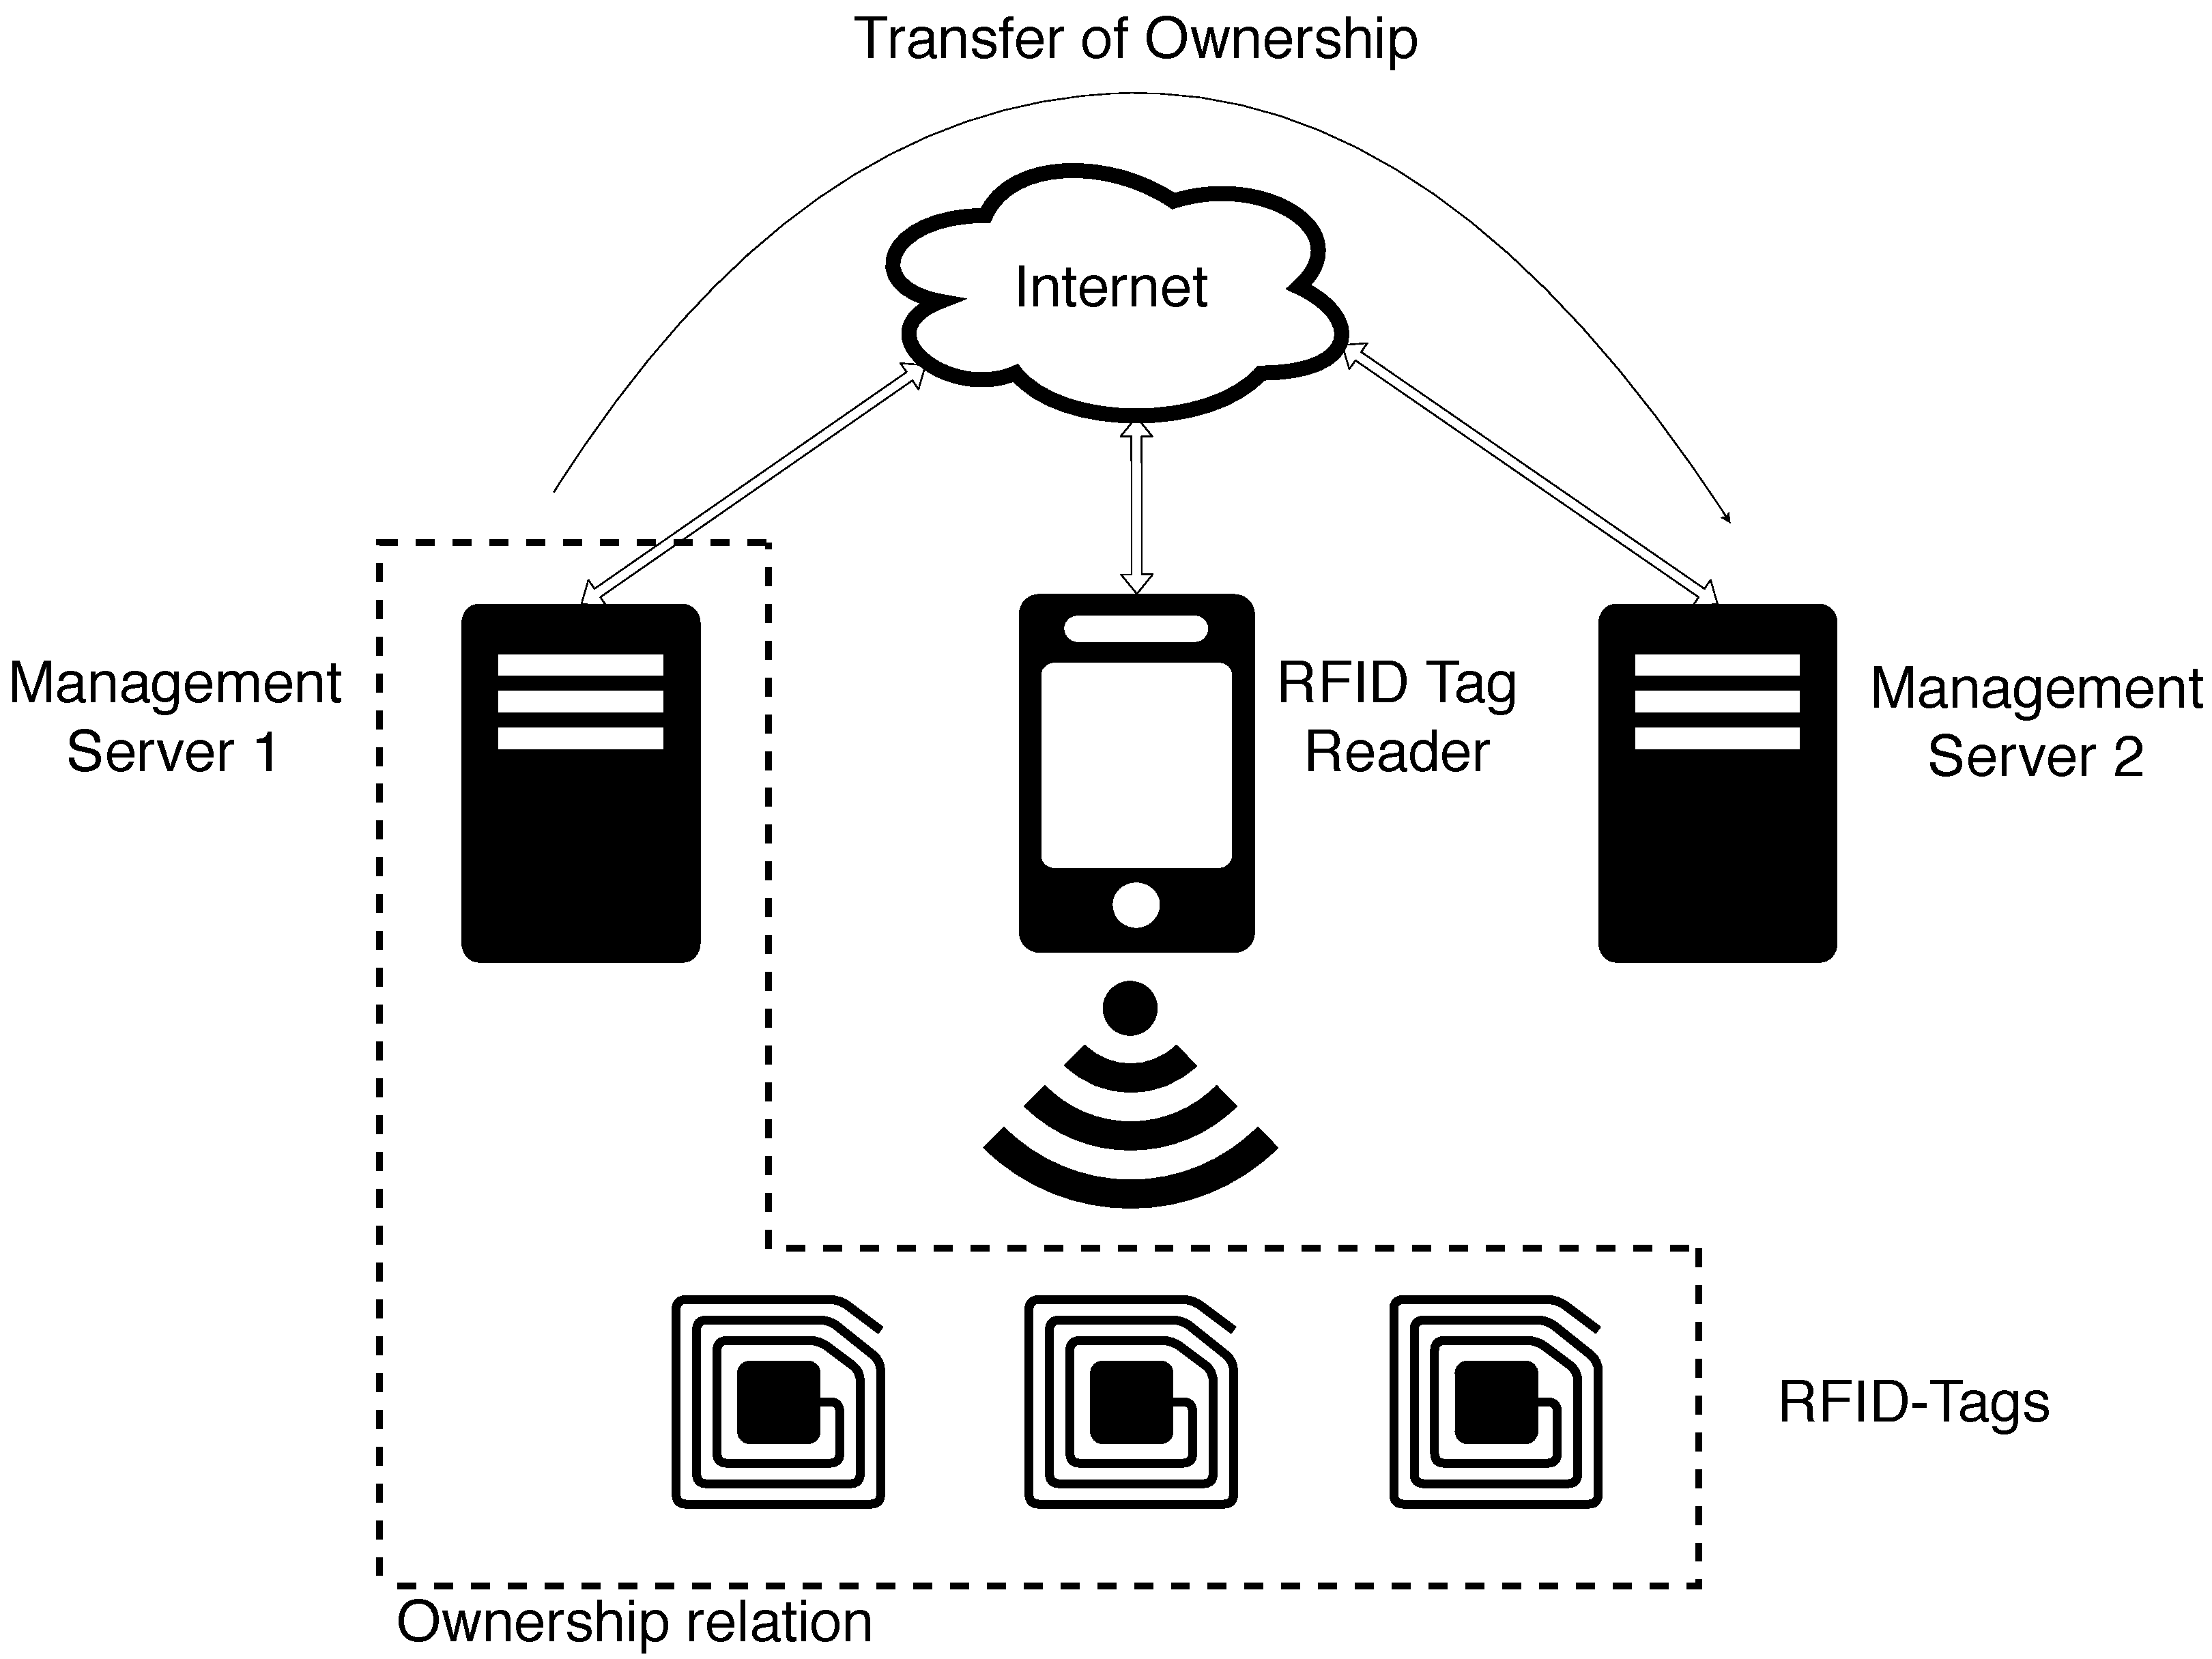
\includegraphics[width=0.9\textwidth]{images/RFID-Tag_OT.pdf}
\caption{RFID-System and ownership transfer}
\label{fig:rfid-ot}
\end{figure}



A recent and comprehensive survey of the research into ownership transfer can be found in \cite{taqieddin2018tag}.
Some ownership transfer solutions for IoT \cite{tam2004protocol}, use public-key encryption to solve this problem straightforwardly. However, constrained systems might not be able to handle the complex computations needed for public-key encryption. Besides the computational issue, not all devices might have the memory needed to store the necessary keys and the code needed to do public-key computations.

In Figure \ref{fig:iot-ot}, we show a schematic overview of an IoT deployment. The Management server does not directly connect to the individual devices, but often communicate over the internet, through some gateway. The presence of the gateway is an essential property of such a system. This gateway sometimes needs to translate protocols and terminate DTLS sessions to work correctly. Since individual IoT devices are connected to the Internet, the attack surface is larger compared to an RFID tag. An attacker must be in proximity to an RFID-tag to be able to communicate with it and to intercept messages. Thus many of the security requirements for RFID-systems can not be directly applied to IoT systems.


\begin{figure}[ht]
\centering
%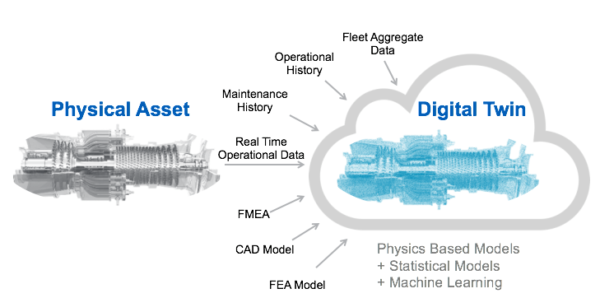
\includegraphics[width=0.9\textwidth]{images/digitial-twin.png}
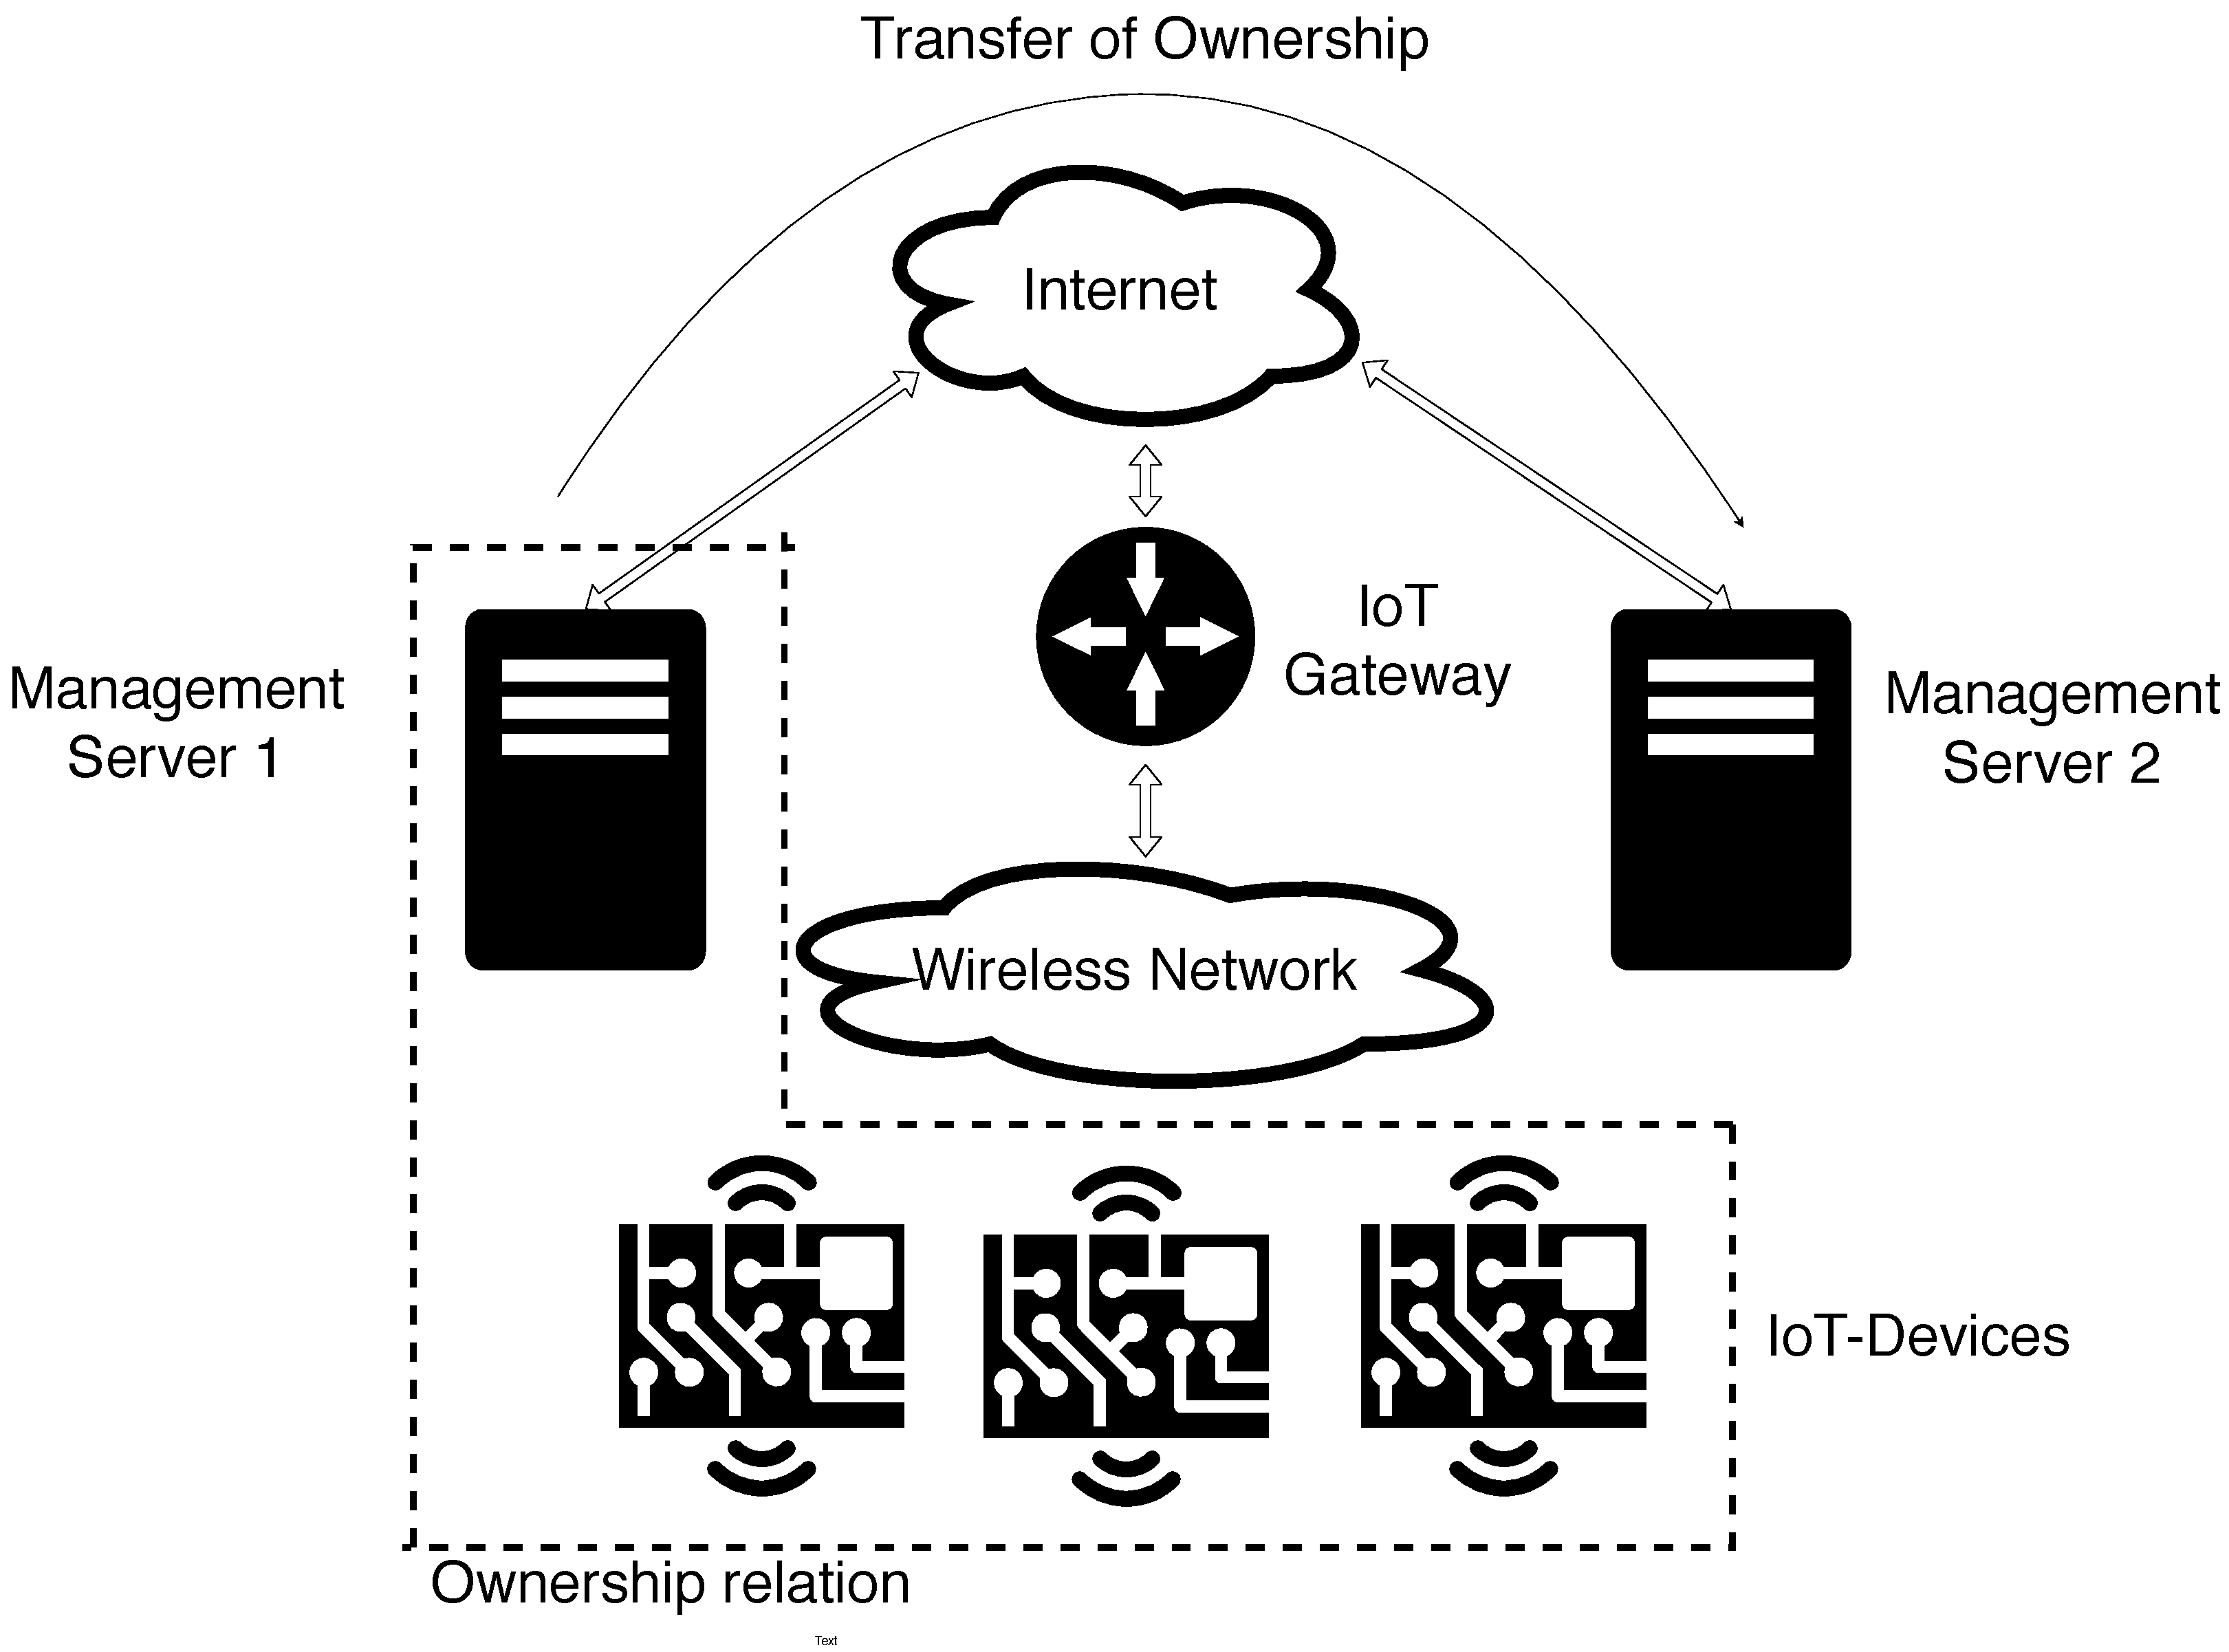
\includegraphics[width=0.9\textwidth]{images/IoT_OT.pdf}
\caption{IoT deployment and ownership transfer}
\label{fig:iot-ot}
\end{figure}


Security requirements for secure ownership transfer protocols are the same as for conventional security protocols. Properties such as confidentiality, integrity protection, availability, and resistance to impersonation attacks are essential to a secure protocol. But then there are new properties that need to be also considered. According to \cite{taqieddin2018tag}, the authors have proposed the security requirements stated below. These requirements apply equally to both RFID-tag solutions and IoT protocols since they are general to the problem of ownership transfer:
\begin{itemize}
    \item New owner privacy: The old owner shall not be able to access data after ownership transfer is completed.
    \item Old owner privacy: The new owner shall be unable to learn anything that the old owner has done before the transfer.
    \item Windowing problem: There shall be no place in time where both the new and the old owner has access to the device at the same time.
    \item Exclusive ownership transfer: It shall be possible to verify that the ownership transfer has gone according to plan.
\end{itemize}
The properties of New owner privacy and Old owner privacy is similar to Forward Security and Backwards Security in a protocol such as TLS. For example, TLS ephemeral keys are negotiated with a key agreement protocol such as Diffie-Hellman \cite{diffie1976new}. Using such a solution work in theory for ownership transfer, but it fails when considering the computational complexity of public-key cryptography. Achieving New owner privacy and Old owner privacy using symmetric cryptography is the challenge here. 

The Windowing problem means that the transfer must be immediate, so there can be no point in time where both the New owner and the Old owner have access to the device that is switching hands. The challenge here is not apparent; when the step that transfers the ownership occurs, it will either succeed or fail. If it completes, then the New owner will have control of the device, but if it fails, the Old owner shall retain control of the device. This has to be done to prevent the device from becoming \emph{orphaned} and left in a state where neither the New owner or the Old owner can access it. 
Exclusive ownership transfer means that the New owner shall be able to verify that devices have been transferred and that they are now under the New owner's control. The requirement here is that the new owner must be able to authenticate all devices after a transfer is complete.

%\cite{RAY2018838}


\section{Digital Twin}
\label{sec:digital_twin}
 Digital Twin is the name given to techniques where a physical device is \emph{mirrored} to a digital copy. This Digital Twin can then be used to perform computations, such as optimizations that can be implemented on the \emph{physical} twin. Several definitions of the term exist, "A Digital Twin is a real-time digital replica of a physical device" is a succinct definition from \cite{bacchiega2019}. Digital Twin as a concept has its origin in aviation manufacturing, where aircraft engines were one of the first applications. The concept was developed during the 1990s and was published in 2002 \cite{grieves2019virtually}. Since then, the application of Digital Twin has spread to Wind Turbines, HVAC (Building Automation), health applications, and many more. 

In Figure \ref{fig:digital-twin}, we show how such a workflow with continuous improvements can look. Academia \cite{boschert2016digital} has studied the concept of continuous simulation.

In \cite{grieves2014digital}\cite{grieves2017digital}, the authors present their idea of how to use Digital Twin to facilitate life-cycle management for complex systems. They discuss how to test, simulate, and improve the physical systems using a Digital Twin. But this is not the only application; many industries and fields investigate what benefits they can get from Digital twin. A summary of these results can be found in \cite{8424832}. 

\begin{figure}[ht]
\centering
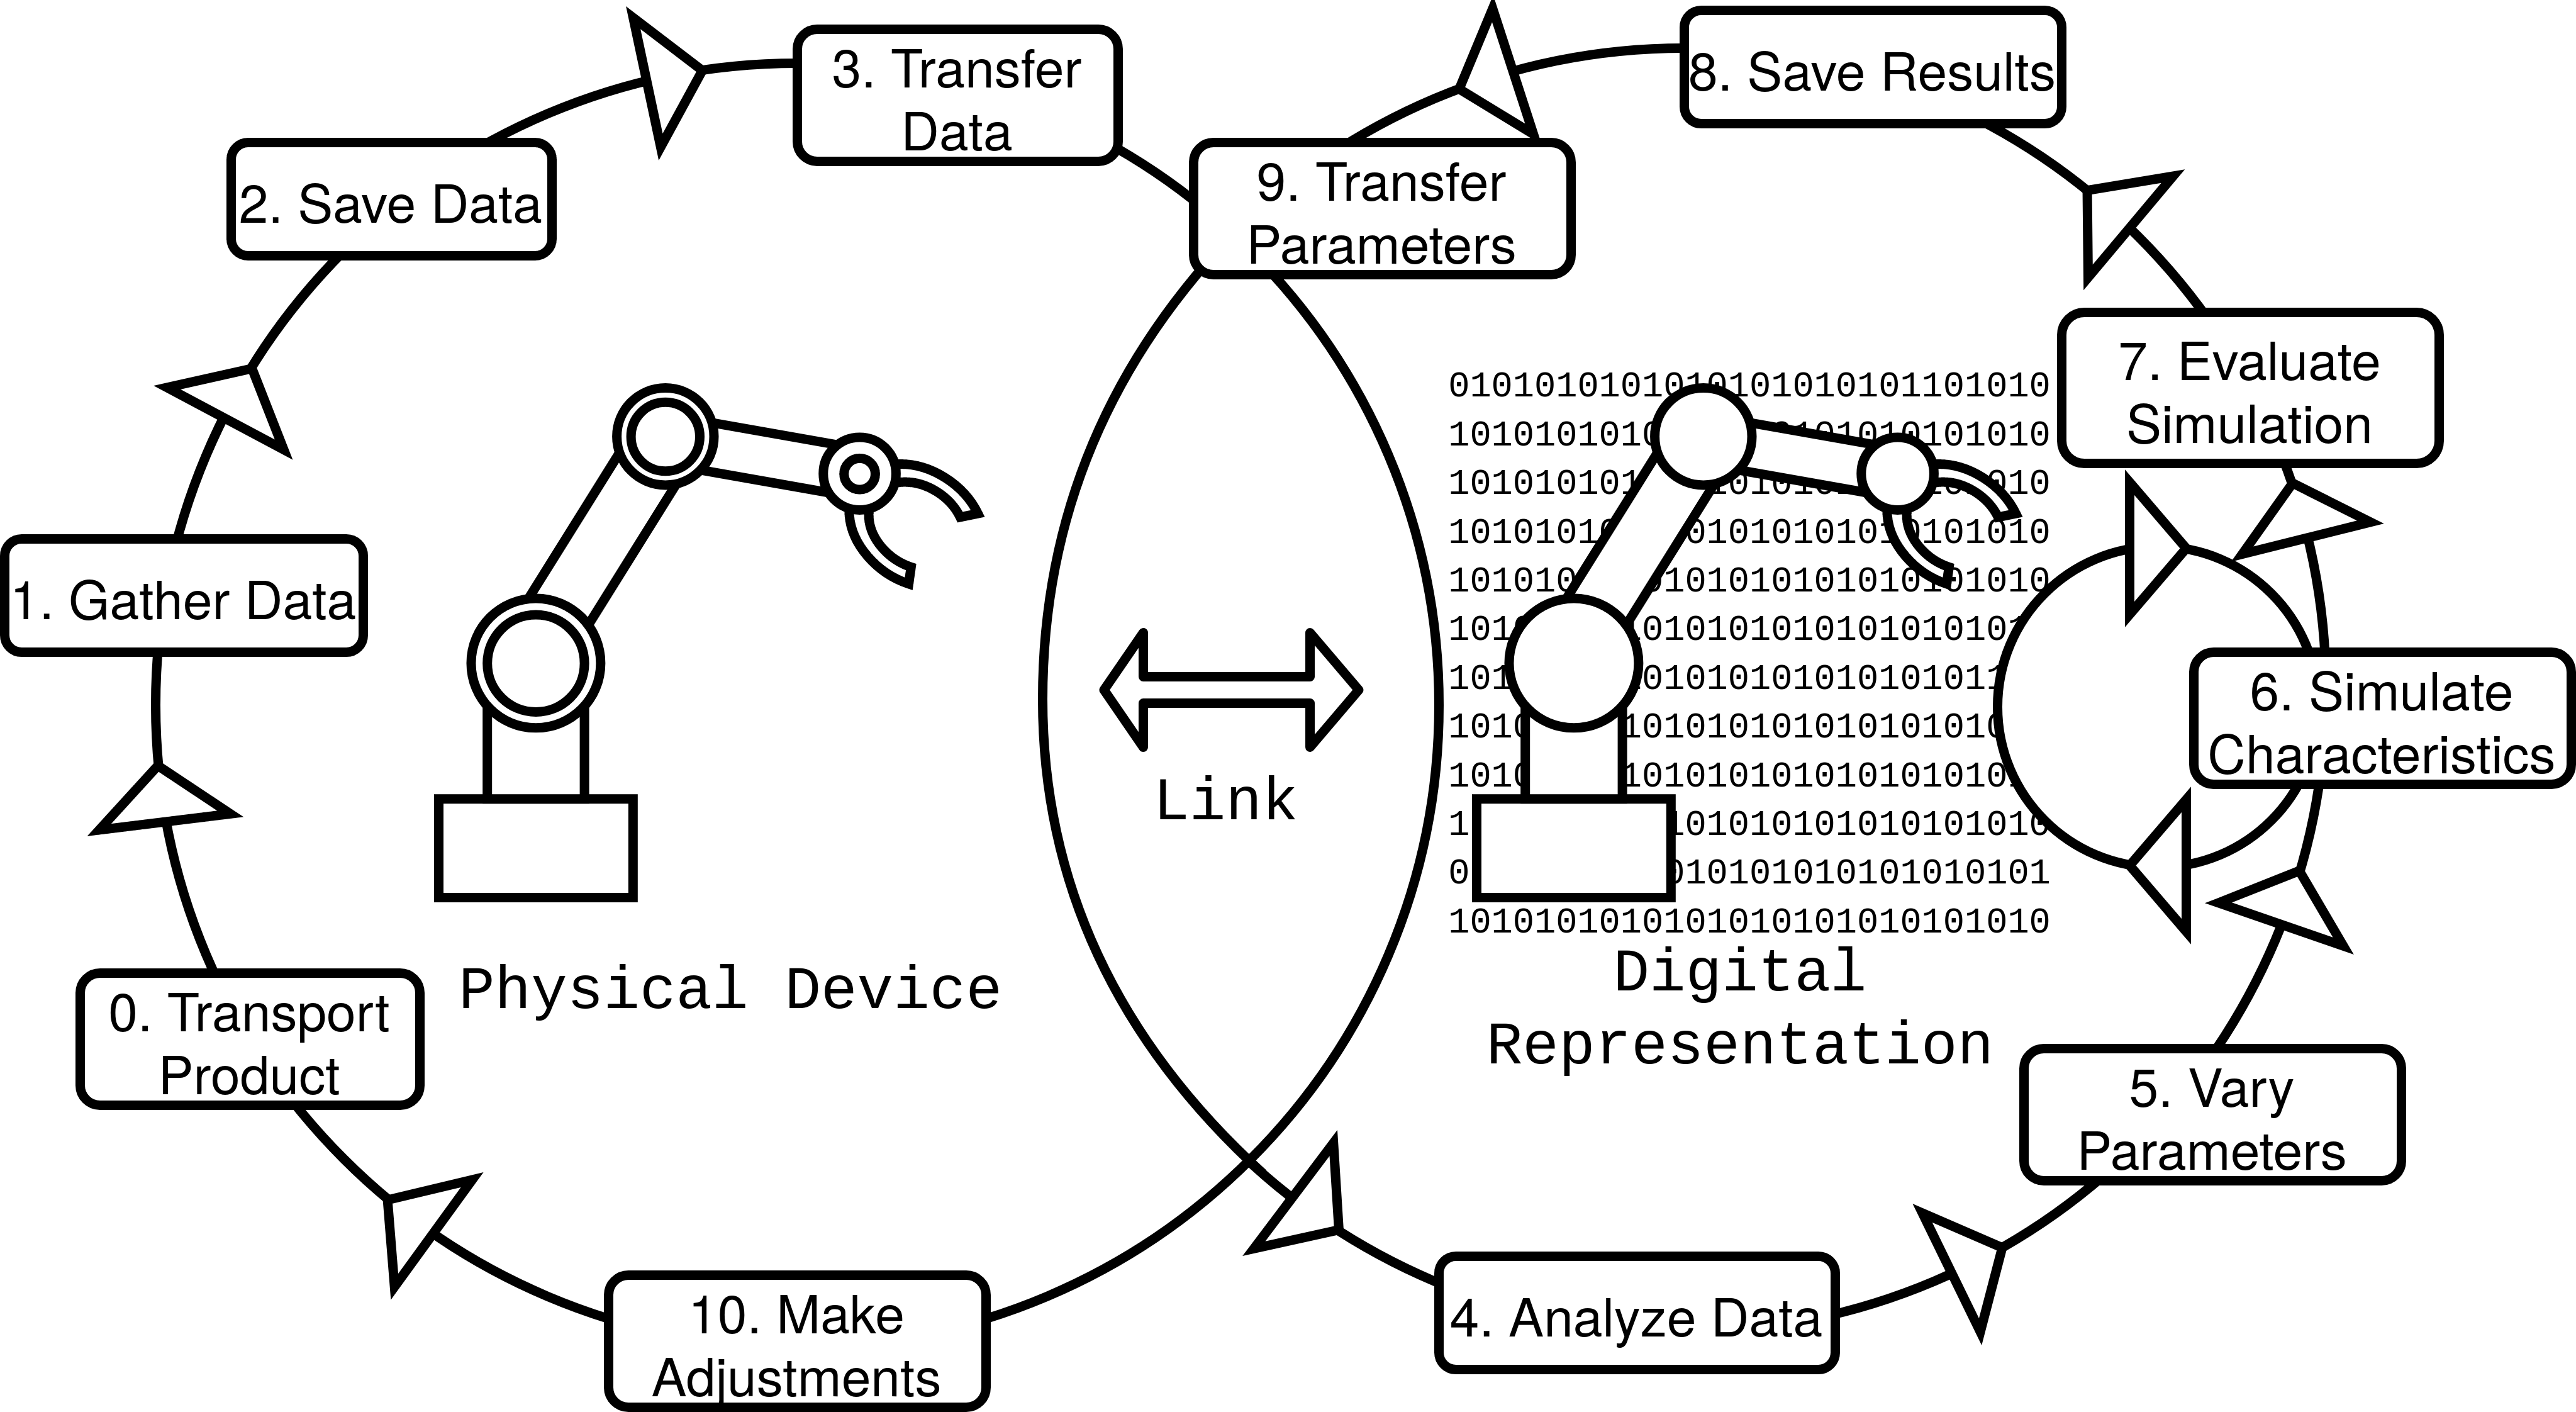
\includegraphics[width=\textwidth]{images/digital_twin.png}
\caption{A schematic representation of a physical device and its Digital Twin surrounded by the workflow of continuous optimization.}
\label{fig:digital-twin}
\end{figure}

Digital Twin can also be used to improve security. In heterogeneous systems, it can be challenging to establish a picture of the system. A Digital Twin of the system can provide such a view. This twin can be used for finding vulnerabilities, both by scanning for known vulnerabilities, static threat modeling and also to create a replica of the system to be used in a \textit{Cyber Range}. 

ICS systems are often so vulnerable to a cyberattack that techniques used in penetration testing such as port scanning can cause systems to crash. Since these systems are connected to a process, a crash is unacceptable, but stopping the process to do a penetration test is usually not possible either. If this penetration test can be made on a \emph{twin} of the system, it would solve both these problems. 

In \cite{bitton2018deriving}, the authors provide a way to generate a Digital Twin of a system that can be used in a penetration test. The Digital Twin can also be used in a cyber range to teach operators of ICS about cybersecurity applied to \emph{their} system.

Digital Twin has been proposed to be useful for many things, such as documentation and continuous improvement. For cybersecurity in industrial control systems and Constrained devices, the ability to synchronize the physical device to a Digital Twin can be used to overcome the limitations we described in Section \ref{sec:cps} and \ref{sec:constrained_devices}.

The ability to replicate a state from a device to a remote entity makes it possible to add functionality to the remote entity. This entity can be a cloud environment, and with a state replication protocol, the results of this added security functionality can be \emph{mirrored} to the physical device. We have investigated such a concept in Paper IV, where we propose a simple state synchronization protocol for use in industrial control systems.

\subsection{State Machine Replication}
Finite-state machines can be used for representing and modeling a variety of computer and automation systems. State machines can also be used to design and specify the behavior of a system. State Machine Replication is a technique to synchronize the states between two or more Finite-state machines \cite{lamport1984using}. 

It might also come as no surprise that computers and automation systems sometimes fail. Adding redundancy to provide fault-tolerance is one way to overcome the problem. By viewing a part of the system as a state machine and then replicating the state to another part of the system, one can achieve redundancy and reducing the probability of a system-wide outage. 


\begin{figure}[ht]
\centering
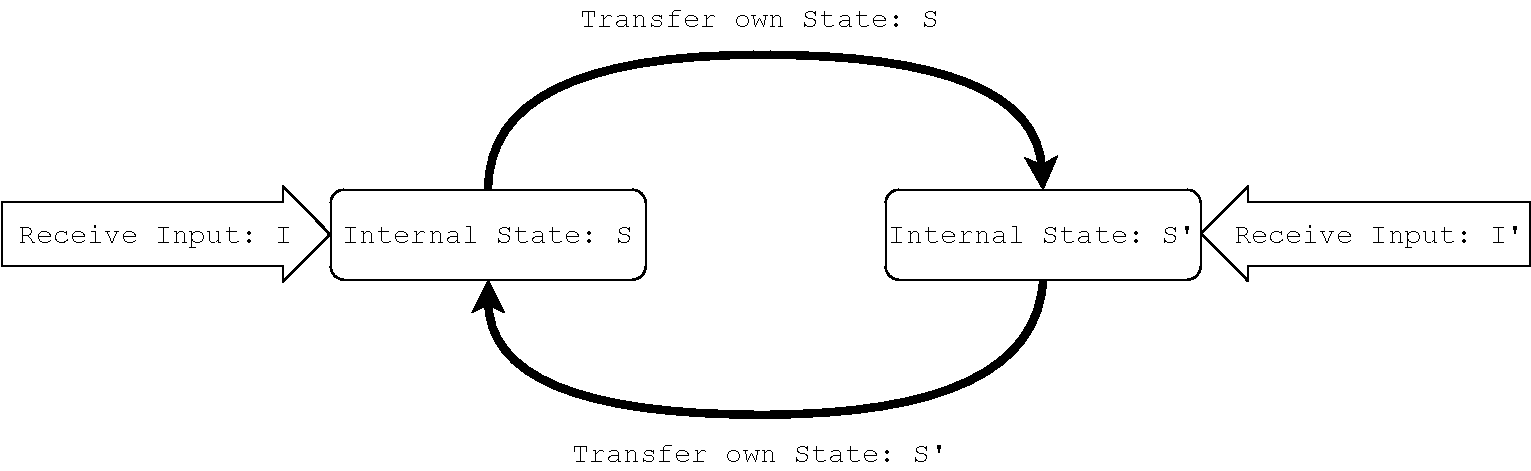
\includegraphics[width=0.9\textwidth]{images/State_replication.pdf}
\caption{A conceptual model of a state replication mechanism}
\label{fig:state-replication}
\end{figure}

As can be read in \cite{charron2010replication}, Replication and State Machine Replication have been investigated for over 30 years. The techniques have been applied to different fields, such as distributed systems and databases. The goal of replication has been both performance gains, by scaling a system and fault tolerance, by duplication of stored data. By mirroring a physical system with a Digital Twin, a new type of application emerges. Here the goal is to provide a single digital image of a system that can be used for further processing.

Above, Digital Twin was defined as "... a real-time digital replica of a physical device", State machine synchronization is one way of achieving \emph{real-time replication}.

Using replication to improve the security of IoT devices has been suggested in \cite{gehrmann2016iot}. The authors present a method to \emph{mirror} an IoT device to a server. The server can provide more extensive security mechanisms than the constrained IoT device. By using a rigid communications protocol that only allows for synchronization between the device and the mirror, a high level of security can be achieved for a constrained device.

The technique of state machine replication has been applied to industrial control systems. In \cite{Eckhart2018}, the authors propose a state replication mechanism to be used for intrusion detection in ICS. The authors use a state replication approach to avoid prohibitive overhead in terms of network and computation overhead in the physical devices.

\begin{figure}[ht]
\centering
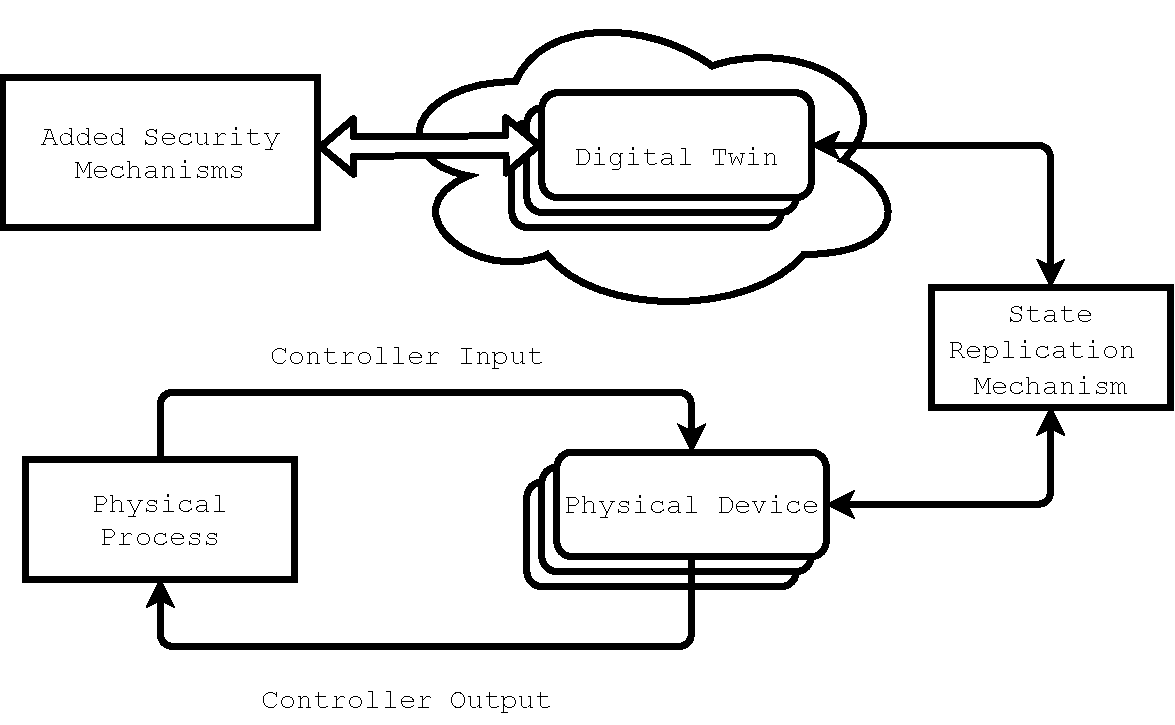
\includegraphics[width=0.9\textwidth]{images/state_replication_security.pdf}
\caption{Adding security mechanism by replicating the physical devices to Digital Twin and perform the complex security mechanisms there.}
\label{fig:state-replication-sec}
\end{figure}

Both \cite{gehrmann2016iot} and \cite{Eckhart2018} propose a similar approach to adding more complex security mechanisms to constrained devices and industrial control systems. In Figure \ref{fig:state-replication-sec}, we show a system overview of such a solution. For constrained devices, this type of solution is attractive because of the limitations in the capabilities we discussed in Section \ref{sec:constrained_devices}. A state synchronization protocol can be implemented with small overhead, so this approach is workable. For ICS, the limitations in available resources that we discussed in Section \ref{sec:cps}, the long lifetimes of devices in ICS, and the complexity of these devices can benefit from the added security mechanisms with the relatively low cost of implementing a State Replication Protocol.

In Paper IV, we have used a State machine synchronization protocol to synchronize a physical device with a Digital Twin. The low overhead of a state machine synchronization protocol makes this an attractive solution to realize a Digital Twin for ICS, considering the limitations described in Section \ref{sec:cps}.

\chapter{Contributions and Conclusions}
\label{ch:coc}
\section{Contributions}
The following sections introduce each contribution, the individual contributions of the author, and the changes made to the publications for print in this thesis.

Author names and acronyms; Martin Gunnarsson (MG), Christian Gehrmann (CG), Joakim Brorsson (JB), Marco Tilcoa (MT), Ludwig Seitz (LS), Francesca Palombini (FP).

%1 OT, 2 Big Data, 3 OSCORE, 4 DT
\subsection{\paperItitle}
\subsubsection{Content}
In this paper, we investigate the problem of Secure ownership transfer. The process of transferring ownership of devices has mainly been studied for RFID-tags but not for IoT devices. The core problem with ownership transfer is \emph{New owner privacy} and \emph{Old owner privacy}. After the transfer of ownership, the new owner shall be unable to learn anything that has happened on the device or any message sent. The old owner shall not learn anything the new owner does after the transfer. 
The work that has been done on Secure ownership transfer for IoT has focused on solutions using public-key cryptography. 
In our intended system, the devices we consider for ownership transfer are Constrained devices, as described in Section \ref{sec:constrained_devices}. Because of the limitations in performance, we have developed a Secure ownership transfer protocol using symmetric-key cryptography.
\subsubsection{Individual Contribution}
MG has together with CG, designed the Secure ownership transfer protocol. CG stated security requirements and, together with MG, did the security analysis of the protocol. MG did the Tamarin model and formal verification of the protocol. MG implemented the experimental evaluation and produced the experimental results.
\subsubsection{For this Thesis}
The paper has been formatted to match the rest of this thesis.


\subsection{\paperIItitle}
\subsubsection{Content}
Wireless sensor networks are being deployed in larger numbers. The data that is sampled is usually sent to a remote server for analytics. This server might be owned by a third party or running in a cloud environment. This is a scenario envisioned in both Industry 4.0 and Industrial IoT, as described in Sections \ref{subsec:i4} and \ref{subsec:wsn_iot}.

Collecting and analyzing data in such a way can provide increase efficiency. However, sending data can reveal secrets about the origin of the data, being either individuals or company secrets in an industrial setting. To solve this privacy problem, we propose a new scheme of identity-privacy for data items. We have described the problem of readable Key Identifiers in Section \ref{sec:object_security}. Our proposed scheme only uses symmetric key operations and is suitable for very constrained sensors of the type we described in Section \ref{sec:constrained_devices}. The proposed protocol uses the concept Object Security that we detailed in Section \ref{sec:object_security}, and encrypts each data item individually. These data items can then be stored intermittently in an encrypted form without extra processing.
\subsubsection{Individual Contribution}
CG designed the protocol with minor input from MG. CG performed the security analysis and defined the property of Identity Privacy. MG wrote the proof-of-concept implementations and performed the performance evaluation.
\subsubsection{For this Thesis}
The paper has been formatted to match the rest of this thesis. Some spelling errors have been corrected. One error in a definition, noticed by a sharp-eyed reader, has been corrected.


\subsection{\paperIIItitle}
\subsubsection{Content}
OSCORE is a protocol recently standardized by the IETF. It is a protocol for Constrained devices that used the Object security concept to protect CoAP messages. We have discussed the limitations of Constrained devices in Section \ref{sec:constrained_devices} and the concept of Object security in Section \ref{sec:object_security}. In this work, we have evaluated the first constrained implementation of OSCORE and compared it against DTLS1.2, the state of the art solution for protecting CoAP messages. 
\subsubsection{Individual Contribution}
MG wrote the constrained OSCORE implementation. MG and JB performed the performance evaluation. All authors, MG, JB, MT, FP, LS, collaborated in writing the background and the description of OSCORE.
\subsubsection{For this Thesis}
The paper has been formatted to match the rest of the thesis.

\subsection{\paperIVtitle}
\subsubsection{Content}
In this paper, we propose a novel security architecture for industrial control systems based on the concept of Digital Twin. Digital Twin is a concept that has been previously used for process simulation and continuous optimization. We have discussed the concept of Digital twin in detail in Section \ref{sec:digital_twin}. 

We propose a way to utilize Digital twin to automate security mechanisms that provide scanning of firmware for vulnerabilities and automated patching of industrial control systems. By using Digital Twin and State machine synchronization, we have shown that it is possible to offload complex security mechanisms to a remote Digital Twin. This can be used to overcome the limitations in industrial control systems that operate under strict real-time deadlines, as we described in Section \ref{sec:cps}. 
\subsubsection{Individual Contribution}
CG designed the Digital Twin replication model and security architecture. CG performed the security analysis. MG implemented the state synchronization protocol and performed the performance evaluation.
\subsubsection{For this Thesis}
The paper has been formatted to match the rest of the thesis.

\newpage

\section{Conclusions}
In this thesis, we have looked at Industrial control systems, cyber-physical systems, and IoT in the context of future industrial applications. Industry 4.0 is a concept where increased connectivity and data-sharing together with new technologies such as cloud computing can increase the productivity of industrial systems. We focused on edge devices in these networks; many such devices are limited in terms of performance and can be categorized as Constrained devices.

We have investigated two main topics of security for these systems; security life cycle management for both industrial control systems and Wireless Sensor nodes and secure communications protocols for Constrained IoT devices. 

On the topic of security life cycle management, we have presented a novel security architecture for industrial control systems using Digital Twin. We have evaluated the state synchronization protocol that synchronizes the physical devices with the Digital Twin and found it to be lightweight and suitable for use in industrial control systems.

We have also presented a protocol to securely transfer the ownership of constrained wireless devices from one owner to a new owner. The protocol uses a Trusted Third Party to enable the use of symmetric cryptography while still providing the desired security properties. The protocol was formally verified to prove that the stated security requirements hold, and it was evaluated in terms of performance. We found it to be suitable for deployment in constrained environments.

On the topic of communications protocols for constrained wireless devices, we have presented two works.

In the first paper, we present a new protocol that provides Identity privacy for sensor data in a wireless sensor network. We show that the proposed protocol can achieve K-anonymity using only symmetric cryptography. The protocol was evaluated on a constrained device and found to have acceptable performance for use in its intended setting.

The second paper on the topic of communications protocols for constrained wireless devices is an evaluation of the OSCORE protocol. We have evaluated the recently standardized protocol OSCORE to the current state-of-the-art method of securing CoAP messages, namely DTLS1.2. We have found that OSCORE performs roughly the same as DTLS in terms of computational complexity, while OSCORE has lower network per-message overhead. 


\label{sec:kappa-conclusions}
{ \raggedright
\printbibliography[segment=\therefsegment,heading=bibintoc]
}
